%\chapter{det-comp}


%%%%%%%%%%%%%%%%%%%%%%%%%%%%%%%%%%%%%%%%%%%%%%
%\section{Anode Plane Assemblies}

%%%%%%%%%%%%%%%%%%%%%%%%%%%%%%%%%%%%%%%%%%%%%%
%\section{Cathode Plane Assemblies}

%%%%%%%%%%%%%%%%%%%%%%%%%%%%%%%%%%%%%%%%%%%%%%
%\section{Field Cage}

%%%%%%%%%%%%%%%%%%%%%%%%%%%%%%%%%%%%%%%%%%%%%%
%\section{HV components}

%%%%%%%%%%%%%%%%%%%%%%%%%%%%%%%%%%%%%%%%%%%%%%
\section{TPC Front-end Electronics}
%\chapter{Cold Electronics}
\label{ch:ce}

%
%%%%%%%%%%%%%%%%%%%%%%%%%%%%%%%%
%\subsection{Introduction}
\subsection{Overview and requirements}
\label{subsec:ce_intro}

\begin{cdrfigure}[The front-end electronics mounted on an APA]{tpcce_FEMBonAPA}{The 
front-end electronics as mounted on an APA.
  {\bf Top:} The front-end electronics is shown in the red circle.
  {\bf Bottom:} Cross section view. Mounting hardware between the front-end electronics 
and the APA fin is not shown.}
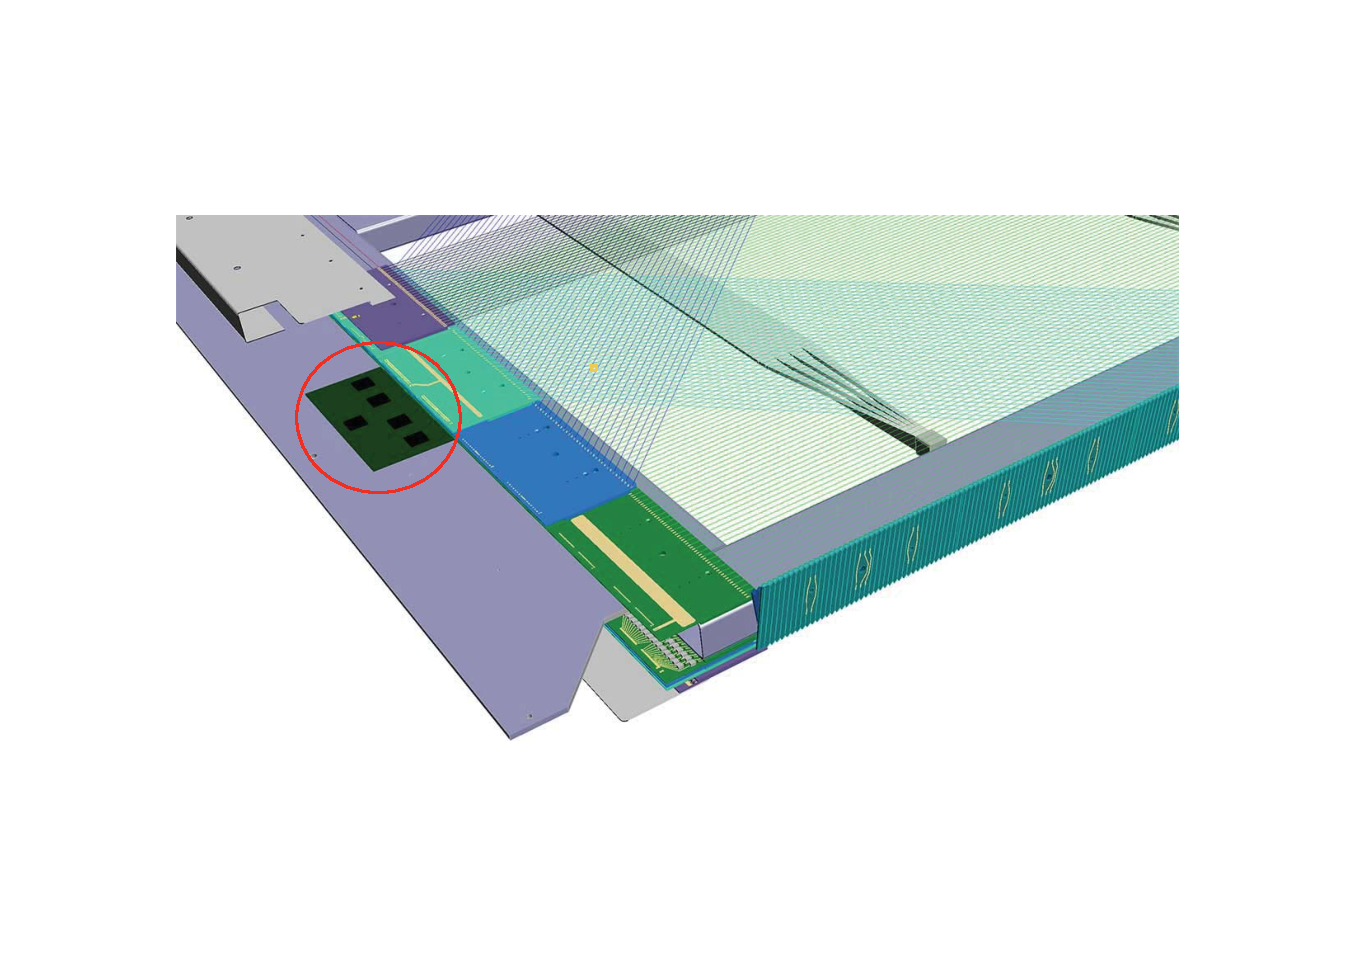
\includegraphics[width=0.8\linewidth]{tpcce_CMBonAPA_1.pdf}
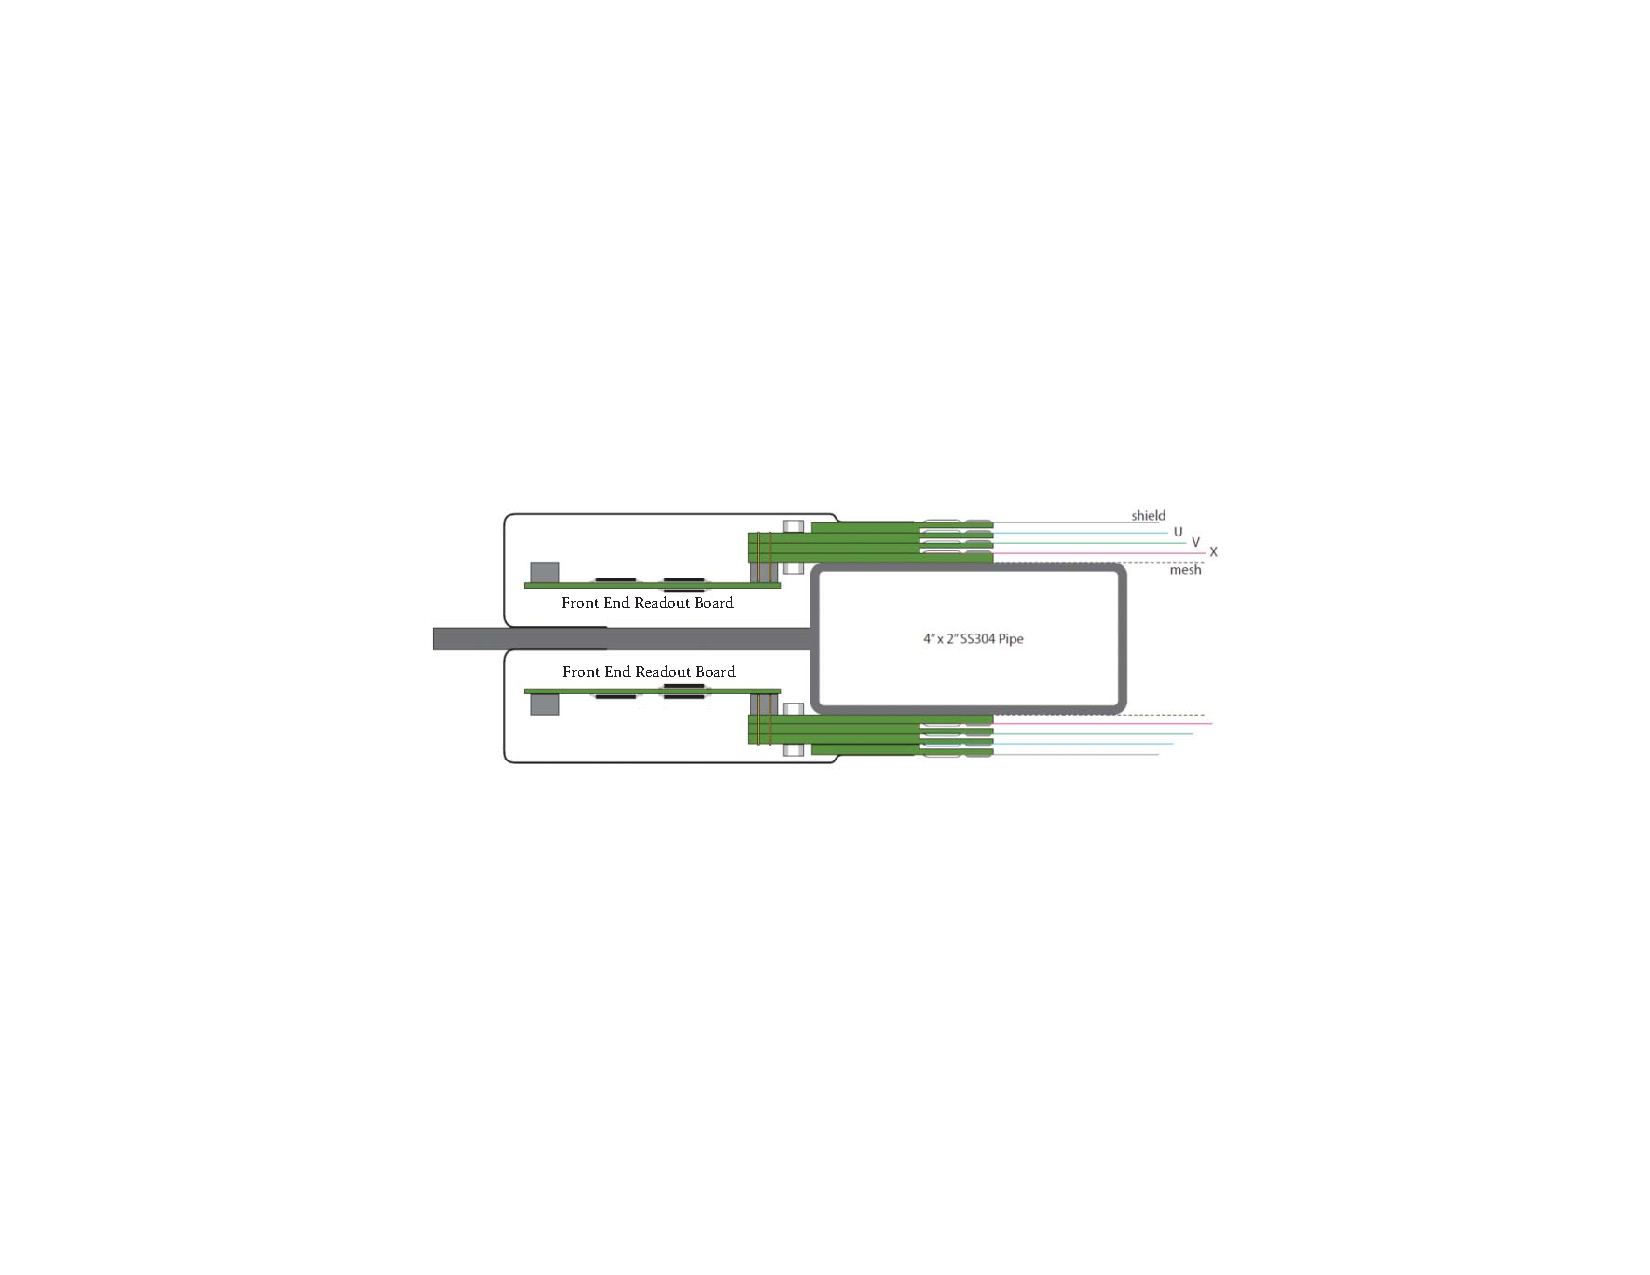
\includegraphics[width=0.8\linewidth]{tpcce_CMBonAPA_2.pdf}
\end{cdrfigure}

The DUNE single-phase TPC read-out electronics are referred to as the ``Cold Electronics'' (CE) because they reside in LAr,
mounted directly on the APA (Figure~\ref{fig:tpcce_FEMBonAPA}).
This reduces channel capacitance and noise by minimizing the length of the connection between an anode wire
and its corresponding electronics input.
The CE signal processing is implemented in ASIC chips using CMOS technology,
which has been demonstrated to perform well at cryogenic temperatures,
and includes amplification, shaping, digitization, buffering, and multiplexing (MUX) of the signals.
The CE is continuously read out,
resulting in a digitized ADC sample from each APA channel (wire) up to every 500~ns (2~MHz maximum sampling rate).

The 2,560 channels from each APA are read out by 20 Front-End Motherboards (FEMBs), each providing 
digitized wire read-out from 128 channels. One cable bundle 
connects each FEMB to the outside of the cryostat via feedthroughs in CE flanges, with single flanges servicing each APA as shown in Figure~\ref{fig:tpcce_apa_flange}. 
Each cable bundle contains wires for low-voltage (LV) power, high-speed data readout,
and clock/digital-control signal distribution.
Eight separate cables carry the TPC wire-bias voltages from the CE flange to the APA wire-bias boards, as
shown schematically in Figure~\ref{fig:tpcce_cr_board}.

\begin{cdrfigure}[Connections between CE flange and APA]{tpcce_apa_flange}{Connections between
the CE flange and APA.}
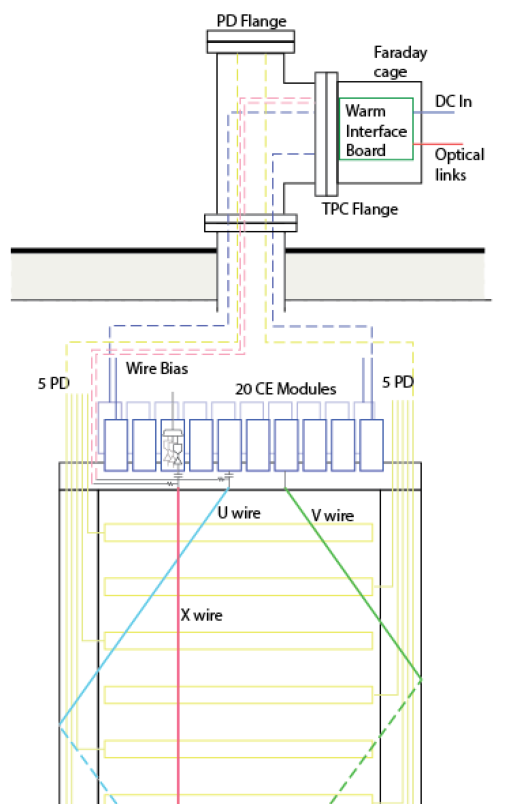
\includegraphics[width=0.4\linewidth]{tpcce_apa_flange.pdf}
\end{cdrfigure}

The components of the CE system are the
\begin{itemize}
\item Front-end mother boards (FEMBs) which house the cold ASICs and are installed on the APAs;
\item Cables for the data, clock/control signals, LV power, and wire-bias voltages 
between the APA and the CE flanges (cold cables);
\item CE flanges with feedthroughs to pass the data, clock/control signals, 
LV power, and APA wire-bias voltages between the inside and outside of the cryostat;
\item Warm electronics crates (WECs) that are mounted on the CE flanges and contain the Warm Interface Boards (WIBs)
and Power and Timing Cards (PTCs) for further processing and distribution of the signals entering/exiting the cryostat;
\item Filter cables for transmitting data and clock/control signals between the WECs and the data acquisition 
(DAQ) and slow control systems;
\item Cables for LV power and wire-bias voltages between the CE flange and external power supplies (warm cables);
\item LV power supplies for the CE and bias-voltage power supplies for the APAs
\end{itemize}

The electrical cables for each APA enter the cryostat through a single 
CE flange, creating an integrated unit that provides local diagnostics for noise and validation testing,
and follows the grounding guidelines in Section~\ref{subsec:groundshield}.

%
%%%%%%%%%%%%%%%%%%%%%%%%%%%%%%%%
%\subsection{Design Considerations} 
%\label{subsec:ce_reqs_n_specs}

The most significant requirements for the CE are listed here. The CE shall:

\begin{itemize}	
\item Provide the means to read out the TPC wires and transmit their data in a useful format to the DAQ.
\item Operate for the life of the facility without significant loss of function.
\item Record the channel waveforms continuously without dead time.
\item Be constructed only from materials that are compatible with high-purity LAr.
\item Provide sufficient precision and range in the digitization to:
\begin{itemize}
\item Discriminate electrons from photon conversions;
\item Optimize the reconstruction of high- and low-energy tracks from accelerator-neutrino interactions;
\item Distinguish a Minimum Ionizing Particle (MIP) from noise with a signal-to-noise ratio $>$ 9:1;
\item Measure  ionization up to 15 times that of a MIP particle, so that stopping kaons from proton decay can be identified.
\end{itemize}
\item Ensure that all power supplies have: 
\begin{itemize}
\item Local monitoring and control
\item Remote monitoring and control through DAQ
\item Over-current and over-voltage protection circuits
\end{itemize}
\item Ensure that the signal feedthroughs are able to withstand twice their nominal operating voltages 
with a maximum specified leakage current in 1-atm argon gas.
\end{itemize}


%%%%%%%%%%%%%%%%%%%%%%%%%%%%%%%%
%\subsubsection{Electrical design}
%\label{subsec:ele_design}
\subsubsection{Grounding and shielding}
\label{subsec:groundshield}

To avoid structural ground loops, the APA frames described in Section~\ref{subsec:apa_frame} 
are insulated from each other. Each frame is electrically connected to the cryostat at a single 
point on the feedthrough board in the CE flange where the cables exit the cryostat. Mechanical suspension of the APAs 
is accomplished using insulated supports. 

The analog portion of the FEMB contains eight front-end (FE) ASICS configured as 16-channel 
digitizing charge amplifiers. Input amplifiers on the ASICs have their Common terminals connected 
to the APA frame.  All power-return leads and cable shields 
are connected to both the Common plane of the FEMB and to the CE flange.

Filtering circuits for the APA wire-bias voltages are locally referenced to the Common plane of the FEMBs through low-impedance 
electrical connections. This approach ensures a ground-return path in close proximity to the 
bias-voltage and signal paths. The close proximity of the current paths minimizes the size of potential loops to further 
suppress noise pickup.

Photon detector signals, described in Section~\ref{sec:pd_system}, are carried directly on shielded, 
twisted-pair cables to the CE flange. The cable shields are connected to the 
cryostat at the PDS feedthrough, and to the PCB shield layer on the photon detectors \fixme{readout boards?}. There is no 
electrical connection between the cable shields and the APA frame except at the CE flange.

%
%%%%%%%%%%%%%%%%%%%%%%%%%%%%%%%%
\subsection{Distribution of APA wire-bias voltages}
\label{subsec:ce_wire_bias}

Each side of an APA includes four wire layers as described in Section~\ref{subsec:apa_phys_desc}. 
The inner-most X-plane layer of wires is nominally biased at +820 Volts, with each wire AC coupled 
to one of the 128 charge amplifier circuits on the FEMB. The V-plane wire layer is effectively biased at zero volts, 
with each wire directly connected to one of the charge amplifier circuits. The U-plane wire layer is nominally 
biased at $-$370 Volts with each wire AC-coupled 
to one of the 128 charge amplifier circuits. The outermost G-plane wire layer,
which has no connection to the charge amplifier circuits, is biased at $-$665 Volts.

Electrons passing through the wire grid must drift unimpeded until they reach the X-plane 
collection layer. The nominal bias voltages are predicted to result in this electrically 
transparent configuration.

As described in Section~\ref{} \fixme{2.1.2} the filtering of wire-bias voltages and AC coupling of wire signals passing
onto the charge amplifier circuits is done on  CR boards that plug inbetween the APA wire-board stacks and FEMBs.

Each CR board includes single R-C filters for the X- and U-plane wire-bias voltages. In addition, each board has 48 
pairs of bias resistors and AC coupling capacitors for X-plane wires, and 40 pairs for the U-plane wires. The coupling capacitors block DC while passing AC 
signals to the CE motherboards.

\begin{cdrfigure}[APA wire bias schematic diagram]{tpcce_cr_board}{APA wire bias 
schematic diagram, including the Capacitance-Resistance (CR) board.}
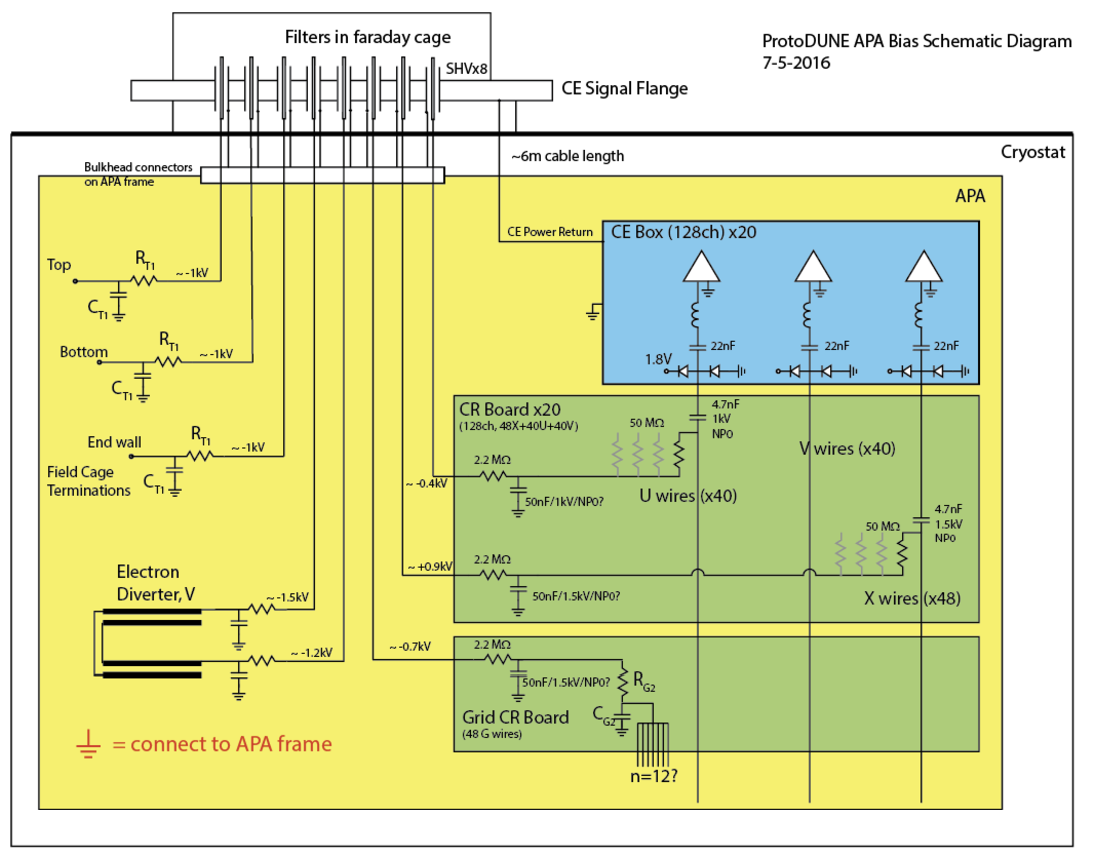
\includegraphics[width=0.9\linewidth]{tpcce_cr_board.pdf}
\end{cdrfigure}

Separate CR boards include a single R-C filter for the G-plane wires and 12 pairs of bias resistors and
coupling capacitors.
Groups of four wires are tied together to share single
bias resistors and filter capacitors. These CR boards do not connect to the charge amplifier circuits on the FEMB.

The amplifier circuits 
have input impedance of 50~$\Omega$ using 22-nF coupling capacitors. 
Clamping diodes limit the input voltage received at the amplifier circuits to between zero and +1.8 Volts.

%%%%%%%%%%%%%%%%%
%\subsubsection{Bias Component Values}
%\label{subsec:bias_comp_values}

Coupling capacitors for the X-plane and U-plane wires are required to block DC bias voltages.
However they also impact the efficiency of the detector circuits.
The sense wires are expected to have 200 pF of capacitance to the APA frame.
Induced or collected charges are effectively divided between the wire capacitance and the coupling capacitor.
To achieve a charge-calibration accuracy of 0.5 percent or better,
the coupling capacitors must be 4.7 nF at ten percent tolerance, or 2.2 nF at five percent tolerance.
Voltage ratings should be at least 1.5 times the expected operating voltages.

Bias resistance values should be at least 20 Meg-ohms to maintain negligible noise contributions.
A target value of 50 Meg-ohms is desired.
The higher value helps to achieve a longer time constant for the high-pass coupling networks.
Time constants should be at least 25 times the electron drift time so that the undershoot in the digitized waveform
is small and easily correctable.
However, leakage currents can develop on PC boards that are exposed to high voltages over extended periods.
If the bias resistors are much greater than 50 Meg-ohms, leakage currents may affect the bias voltages applied to the wires.

The bias-voltage filters are R-C low-pass networks.
Resistance values should be much smaller than the bias resistances to control crosstalk between wires
and limit the voltage drop if any of the wires becomes shorted to the APA frame.
A value around 2.2 Meg-ohms is desired.
Smaller values may be considered although a larger filter capacitor would be required to maintain a given level of noise reduction.
A target value of 47 nF has been established for the filter capacitors.

For the grid-plane bias filters, component values are less critical.
If possible they will be identical to those used for the bias resistors and coupling capacitors
(50~M$\Omega$ and 2.2 to 4.7~nF).


%%%%%%%%%%%%%%%%%%%%%%%%%%%%%%%%
\subsection{Front-End Mother Board}
\label{subsec:fe_arch}

The main component of the CE architecture illustrated in Figure~\ref{fig:tpcce_schem} is the 
128-channel FEMB, which itself consists of an analog motherboard and an attached FPGA 
mezzanine card for processing the digital outputs.
Each APA is instrumented with 20 FEMBs, for a total of 2,560 channels per APA.
The FEMBs plug directly into the APA CR boards, making the connections from the U- and V-plane induction wires and 
X-plane collection wires to the charge amplifier circuits as short as possible.

The analog mother board is instrumented with eight 16-channel FE ASICs,
eight 16-channel ADC ASICs, LV regulators, and input-signal protection circuits.
The 16-channel FE ASIC provides amplification and pulse shaping.
The 16-channel ADC ASIC comprises  12-bit digitizers performant at speeds up to 2 MS/s, local buffering,
and an 8:1 multiplexing (MUX) stage with two pairs of serial readout lines in parallel.

 
   (Figure~\ref{fig:tpcce_CMBpix}).
% following pgraph moved up 9/27   
Each FE ASIC channel has a charge amplifier circuit with a gain selectable from one of 4.7, 7.8, 14 and 25~mV/fC
(full scale charge of 55, 100, 180 and 300~fC),
a high-order anti-aliasing filter with adjustable time
constant (peaking time 0.5, 1, 2, and 3 $\mathrm{\mu}$s),
an option to enable AC coupling,
and a baseline adjustment for operation with either the collecting (200~mV) or the non-collecting (900~mV) wires.
Shared among the 16 channels in the FE ASIC are the bias circuits, programming registers,
a temperature monitor, an analog buffer for signal monitoring, and the digital interface.
The estimated power dissipation of FE ASIC is about 6~mW per channel at 1.8~V supply.

The FE ASIC layout is shown in Figure~\ref{fig:tpcce_ADC_ASIC}.
The ASIC was implemented using the commercial CMOS process (0.18~$\mu$m and 1.8~V), which 
is expected to be available for at least another 10~years. 
The charge amplifier input MOSFET is a p-channel biased at 2~mA with a L/W (channel length/width) ratio
of 0.27~$\mu$m / 10~$\mu$m, followed by dual cascade stages.
The charge amplification and shaping filter have digitally programmable gain and peaking time
(as specified in Section~\ref{subsec:fe_arch}).
Each channel also implements a high-performance output driver,
which can be used to drive a long cable, but is disabled when interfaced to an ADC ASIC to reduce the power consumption.
The ASIC integrates a band-gap reference (BGR) to generate all the internal bias voltages and currents.
This guarantees a high stability of the operating point over a wide range of
temperatures, including cryogenic.
The ASIC is packaged in a commercial, fully encapsulated plastic QFP 80 package.

Prototypes have been evaluated and characterized at RT (300~K) and LN2 (77~K) temperature.
During testing the circuits have been cycled multiple times
between the two temperatures and operated without any change in performance.
Figure~\ref{fig:tpcce_shaper_out} shows the measured pulse response, both as a function
of temperature and the programmable settings of the chip.
These results are in close agreement with simulations and indicate
that both the analog and the digital circuits and interface operate as
expected in a cryogenic environment.

\begin{cdrfigure}[Measured pulse response with details]{tpcce_shaper_out}{Measured pulse response with
 details on gain, peaking time and baseline adjustments}
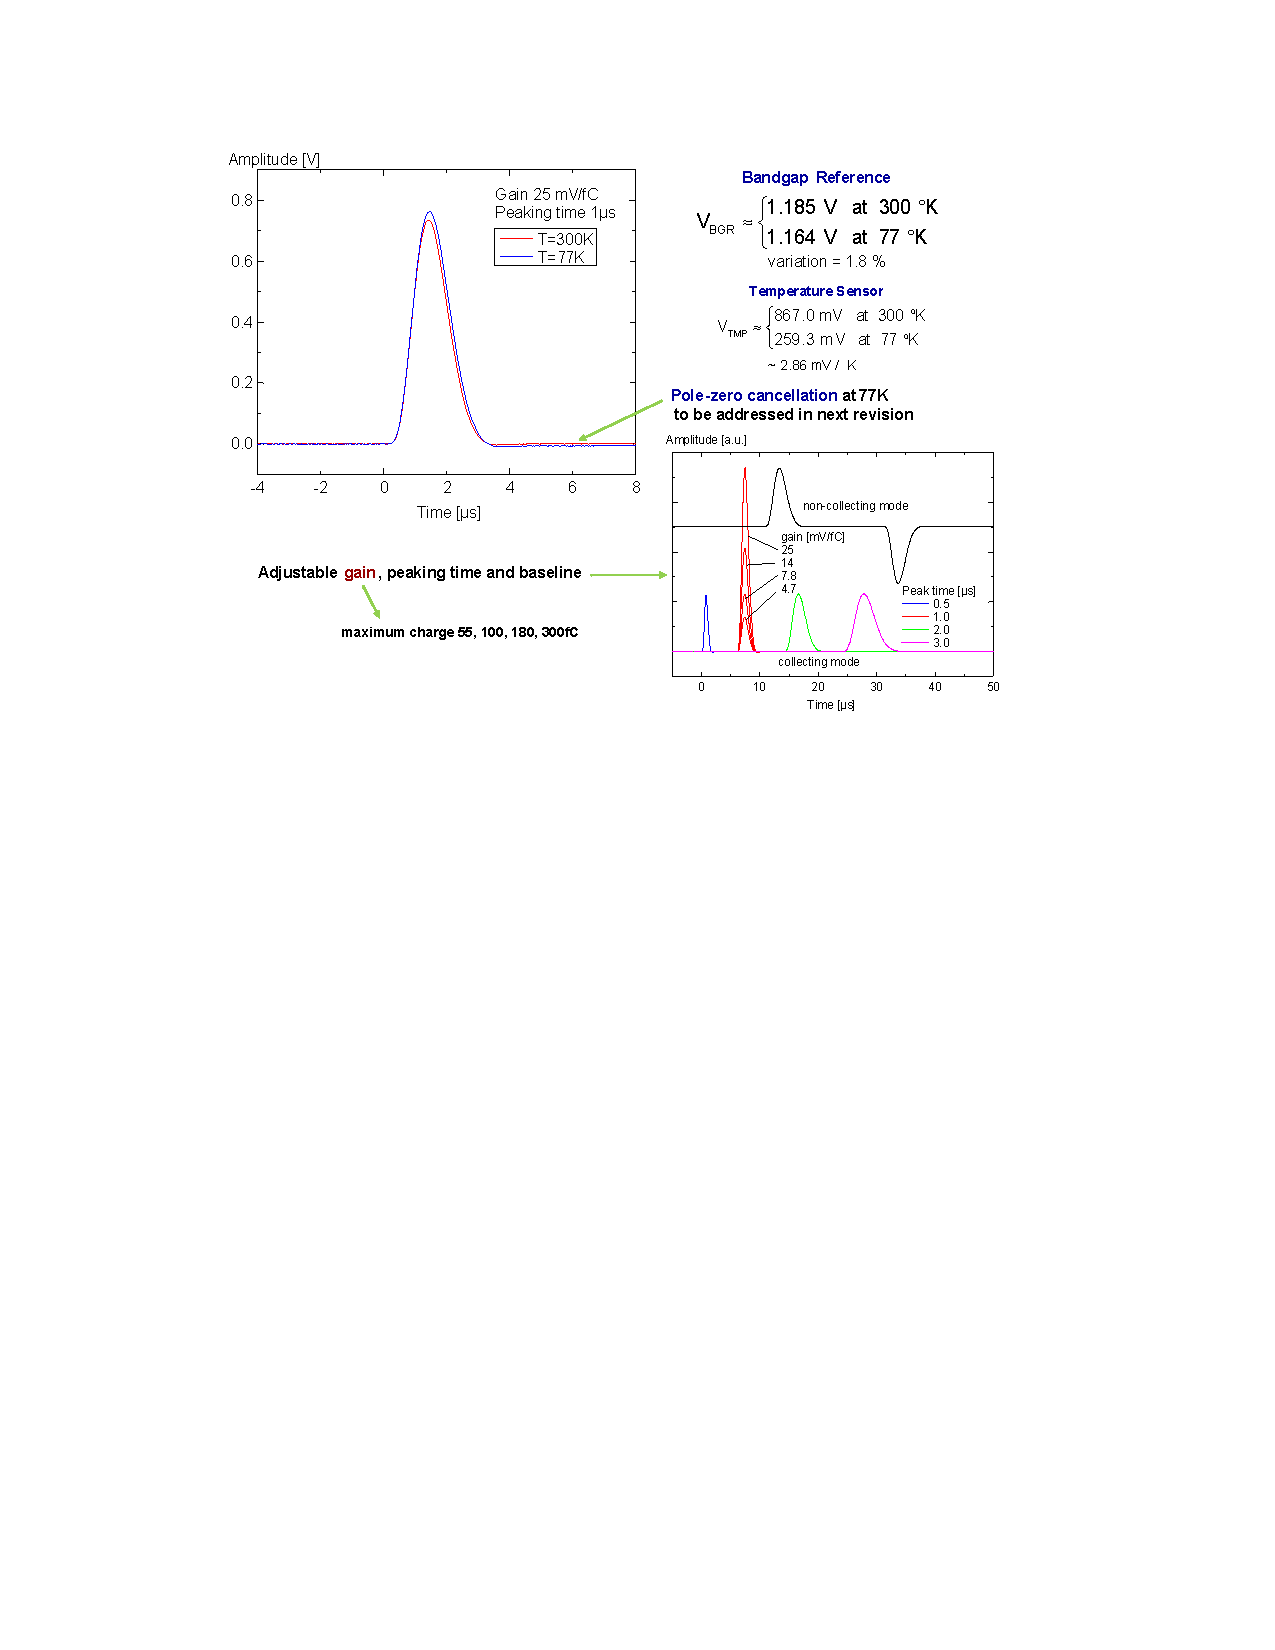
\includegraphics[width=\linewidth]{tpcce_shaper_out.pdf}
\end{cdrfigure}

\begin{cdrfigure}[Measured ENC vs filter time constant]{tpcce_enc}{
Measured ENC vs filter time constant from the latest prototype version of the FEMB
for two different gains, 14~mV/fC and 25~mV/fC. RT = room temperature and 
LN2 = liquid nitrogen}
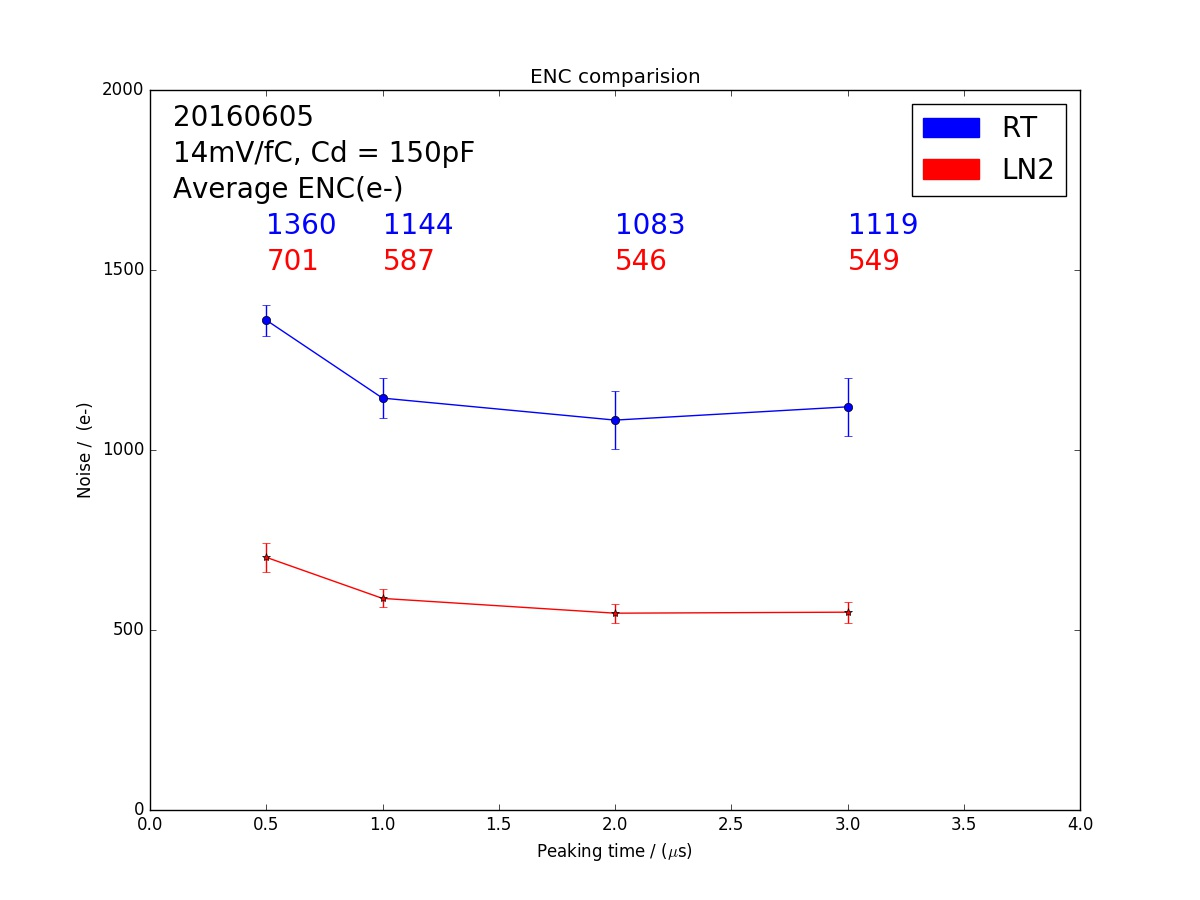
\includegraphics[width=0.45\linewidth]{tpcce_enc_14mV.jpg}
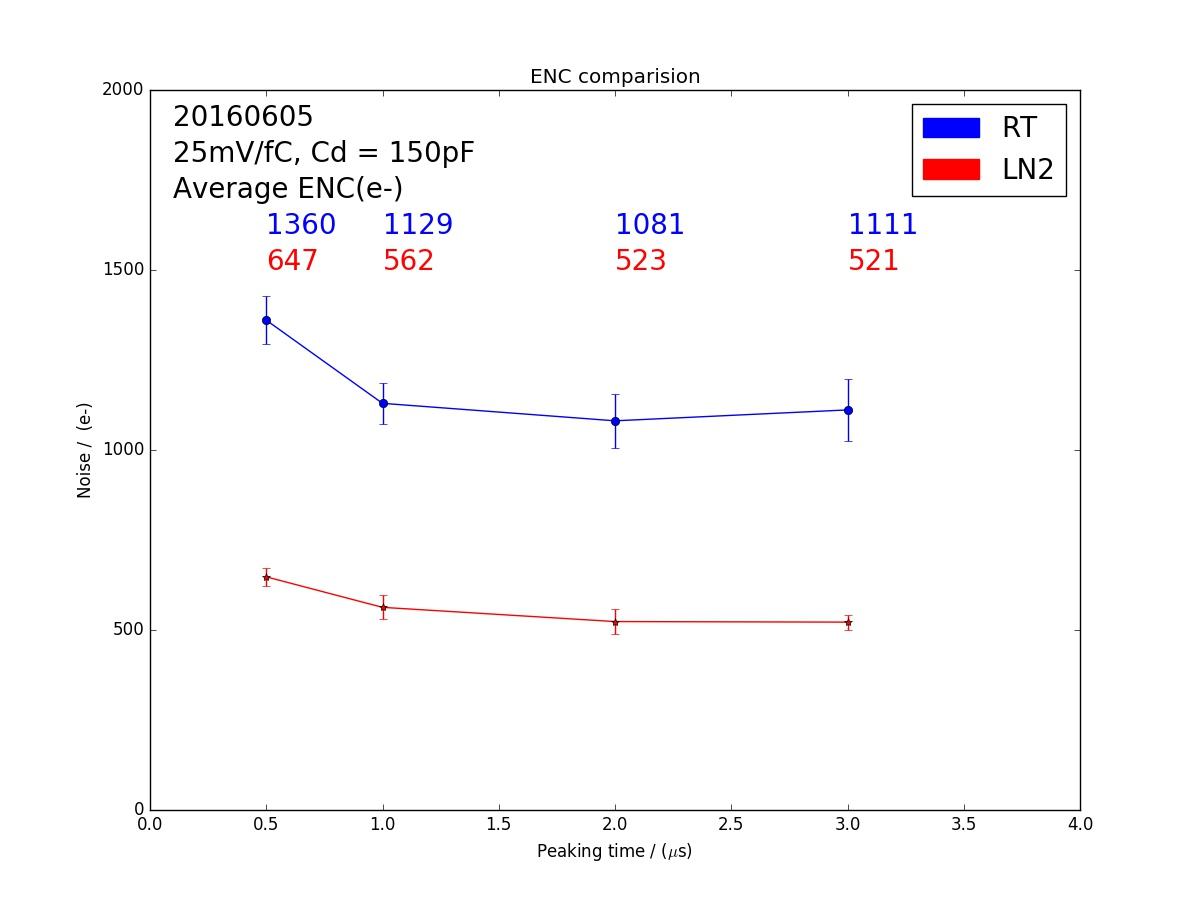
\includegraphics[width=0.45\linewidth]{tpcce_enc_25mV.jpg}
\end{cdrfigure}

Figure~\ref{fig:tpcce_enc} shows the measured Equivalent Noise Charge (ENC) versus 
filter-time constant (peaking time) for two different gains, where ENC is the value of charge 
(in electrons) injected across the detector capacitance that would produce at the output of the 
shaping amplifier a signal whose amplitude equals the output R.M.S. noise. These measurments
were made with prototype FEMBs at both RT and submerged in LN2 with a wire-simulating input capacitance of $C_f~=~150$~pF.
In LN2, for peaking times $>$1~$\mu$s less than 600~e$^{-}$ was measured. For comparison,
a MIP travelling perpendicularly to the wire plane in the direction of wire spacing is
expected to deposit $\sim$~10,000~e$^{-}$ on the collection wires, for a worst-case
S:N$\sim$16:1.

Each channel is equipped with an injection capacitor which can be used
for test and calibration and can be enabled or disabled through a
dedicated register. The injection capacitance has been measured using 
a calibrated external capacitor. The measurements show
that the calibration capacitance is extremely stable, changing from
184~fF at RT to 183~fF at 77~K. This result and the measured
stability of the peaking time demonstrate the high stability of the
passive components as a function of temperature. Channel-to-channel and chip-to-chip
variation in the calibration capacitor are typically less than 1\%. 

The ADC ASIC design is also implementd using the CMOS process (0.18~$\mu$m and 1.8V).
The layout of the ADC ASIC is shown in Figure~\ref{fig:tpcce_ADC_ASIC}. 
The ADC ASIC is a complex design with 320,000 transistors, while the FE ASIC has 16,000.
The transistor design work has been done following the rules for long cryo-lifetime.
Shared among the 16 channels in the ADC ASIC are the bias circuits, programming registers,
an 8:1 MUX, and the digital interface.
The estimated power dissipation of FE ASIC is below 5~mW per channel at 1.8~V supply.
  

\begin{cdrfigure}[The layout of the 16-channel ADC ASIC]{tpcce_ADC_ASIC}{The layout of the 16-channel ADC ASIC}
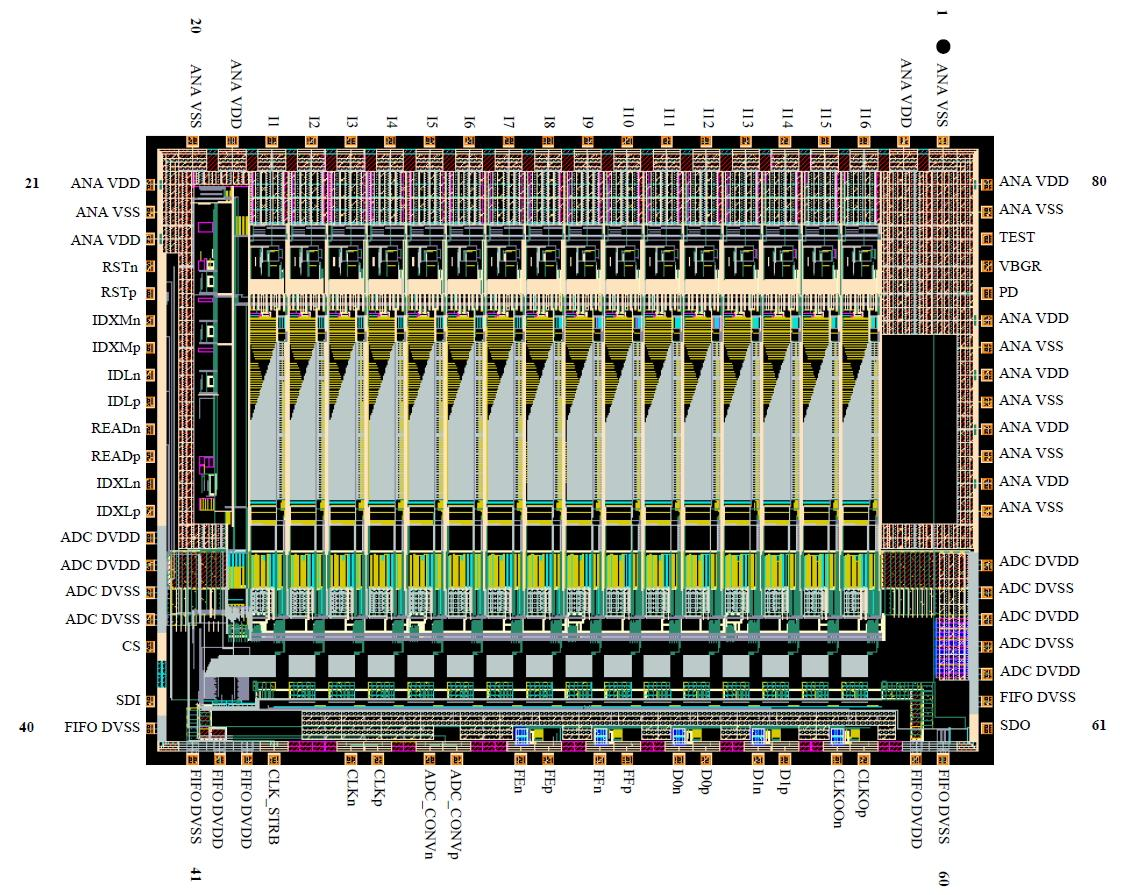
\includegraphics[width=\linewidth]{tpcce_ADC_ASIC_pinout.jpg} % New one
\end{cdrfigure}

The ADC ASIC has an input buffer with offset compensation to match the output of the FE ASIC.
The input buffer first samples the input signal (with a range of 0.2~V to 1.6~V),
then provides a current output after compensating for offset voltage error.
This current output is then supplied to the ADC which converts the input to digital in two phases.
The MSB (Most Significant Bit) 6~bits are first determined followed by the LSB (Least Significant Bit) 6~bits.
After the conversion the thermometer code is converted to binary and latched.
The output of ADC channel 16 can be monitored externally.
The data from the 16 ADCs are transferred in parallel to the FIFO block.
The built-in FIFO is 32~bits wide and 192~bits long,
and has full and empty indicator flags, needed for interfacing to the FPGA.
The ADC along with the input buffers are biased internally using a bias generator and a bandgap voltage reference.
The bandgap voltage (VBGR) can be monitored and/or controlled externally.
It can be put in the low-power sleep mode, and woken up in less than 1~$\mu$s.

Prototypes have been evaluated and characterized at RT (300~K) and LN2 (77~K) temperature.
During these tests the circuits have been temperature-cycled multiple times.
The effective resolution with reference to the input referred noise is $\sim$11.6~bits at both 300~K and 77~K.
The differential non-linearity (DNL) is less than 4 LSBs for 99\% of ADC bins at both 300~K and 77~K.

 
 
 The ACD outputs are passed to the FBGA mezzanine board for transmission to the warm electronics
 located on the outside of the CE flange.

\begin{cdrfigure}[The CE Architecture]{tpcce_schem}{The CE Architecture. The basic unit is the 128-channel FEMB.}
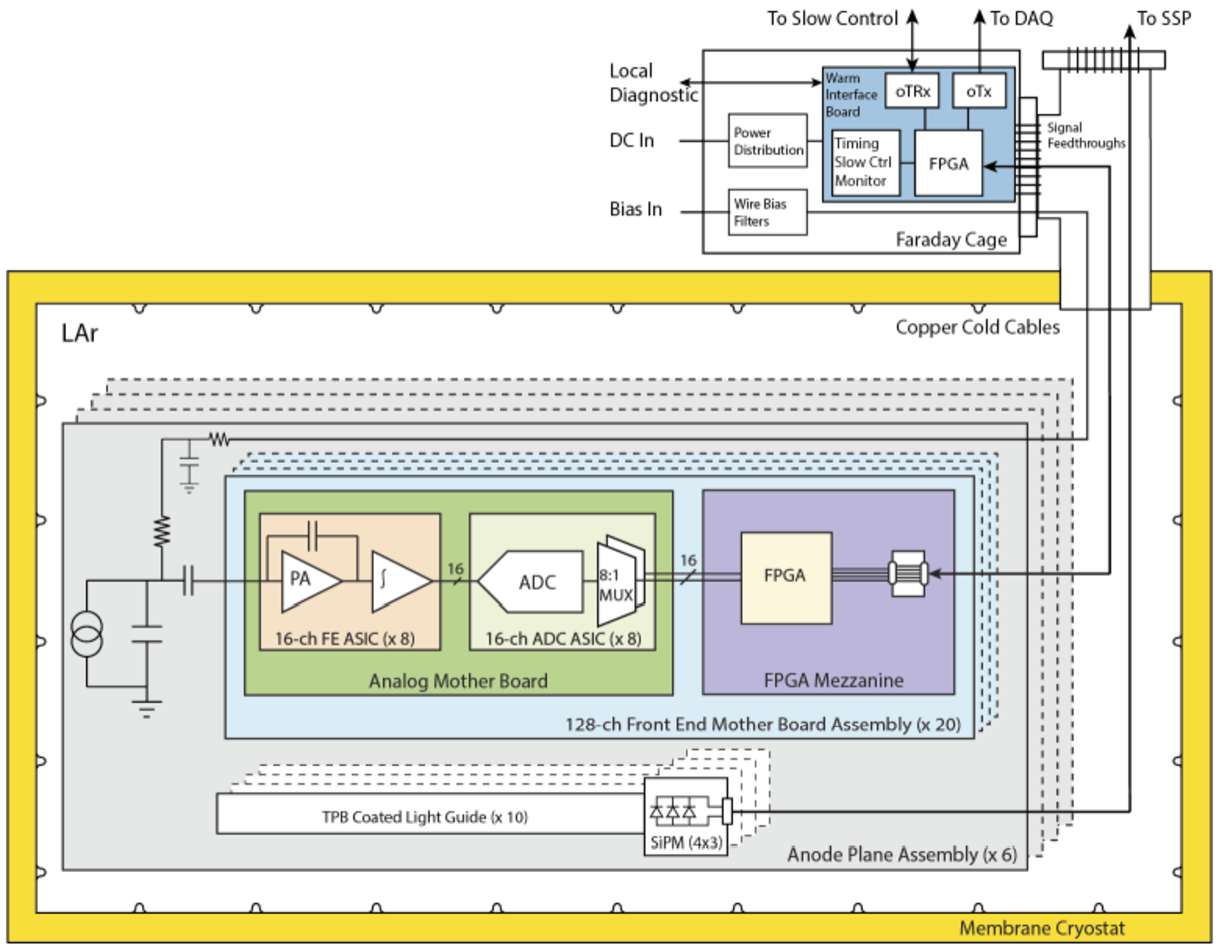
\includegraphics[width=0.9\linewidth]{tpcce_schem.pdf}
\end{cdrfigure}

\begin{cdrfigure}[The Front End Mother Board (FEMB), as used in an early set of tests]{tpcce_CMBpix}
{The Front End Mother Board (FEMB), as used in the early set of tests.
  {\bf Top:} The analog mother board, showing four ADC ASICs and four FE ASICs surface mounted.
  The other side of the board has another four ADC and FE ASICs.
  Except for anticipated small modifications, this board is essentially the final version.
  {\bf Middle:} The FPGA mezzanine, used in place of the digital ASIC mezzanine for the early set of tests.
  {\bf Bottom:} The complete FEMB assembly as used in the early set of tests.
  The cable shown in the high-speed data, clock, and control cable.}
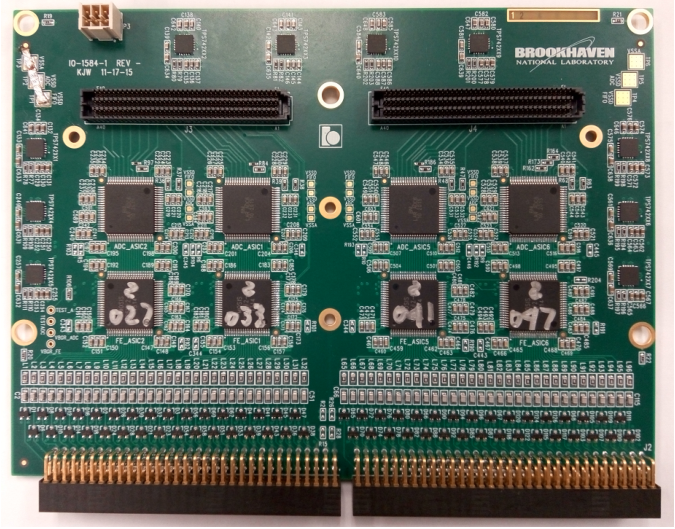
\includegraphics[width=0.65\linewidth]{tpcce_CMBpix_1.pdf}
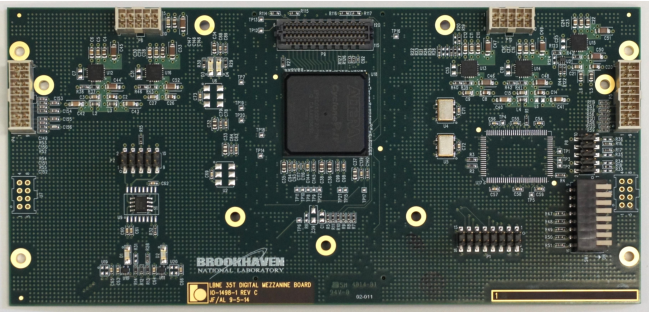
\includegraphics[width=0.65\linewidth]{tpcce_CMBpix_2.pdf}
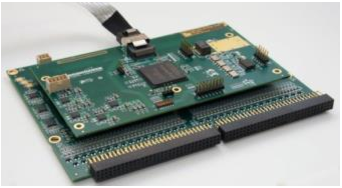
\includegraphics[width=0.45\linewidth]{tpcce_CMBpix_3.pdf}
\end{cdrfigure}


The FPGA has four 4:1 MUX circuits that combine the 16 serial lines from the eight ADC
channels into four serial lines of 32 channels each, and 
four $\sim$1.2 Gigabit-per-second (Gbps) serial drivers that drive the data in each
line over the cold cables to the WIBs.


The data is passed through the CE flange to the WIBs on copper cables utilizing LV differential signaling (LVDS).
On the WIBs, the data is further multiplexed by 4:1 and transmitted over optical
fiber to the DAQ system described in section~\ref{sec:DAQ_online_interface}.


The FPGA on the mezzanine card is also responsible for communicating with the
DAQ and timing systems and providing the clock and control signals required by the FE and ADC ASICs.


Each FEMB is enclosed in a Faraday box to provide shielding from noise. 
As shown in Figure~\ref{fig:tpcce_box}, the Faraday box is designed to make the electrical connection 
between the FEMB and the APA frame, as defined in Section~\ref{subsec:ele_design}. Mounting 
hardware inside the Faraday box connects the common plane of the FEMB to the box casing. The
box casing is electrically connected to the APA frame via twisted conducting wire (not 
shown in Figure~\ref{fig:tpcce_box}). This is the only point of contact between the FEMB and
APA, except for the input amplifier circuits connected to the CR board, which also terminate to
ground at the APA frame, as shown in Figure~\ref{fig:tpcce_cr_board}.

\begin{cdrfigure}[Faraday box for the FEMB]{tpcce_box}{Faraday box for the FEMB.}
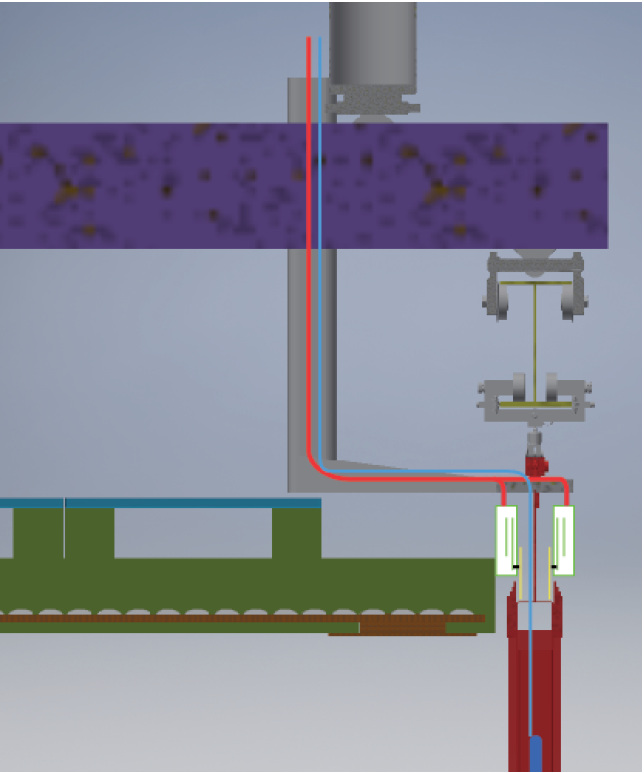
\includegraphics[width=3in]{tpcce_box_1.pdf}
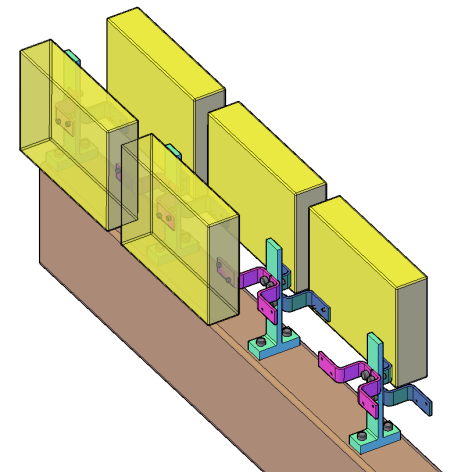
\includegraphics[width=3in]{tpcce_box_2.pdf}
\end{cdrfigure}

%
%%%%%%%%%%%%%%%%%%%%%%%%%%%%%%%%
\subsection{Signal feedthroughs and cold cables}
\label{subsec:ce_feedthrough}

All cold cables originating from inside the cryostat connect to the outside warm electronics through PCB board feedthroughs
installed in the CE flanges that are distributed along the cryostat roof (Figure~\ref{fig:tpcce_FT_InternalCableRoute}).
The TPC data rate per APA, with an overall 32:1 MUX and 80 $\sim$1~Gbps data channels per APA,
is sufficiently low that the signals can be driven over copper LVDS tansmission lines.
Additional LVDS transmission lines are available for the distribution of clock signals and control information,
which are transmitted at a lower bit rate.
Optical fiber is employed externally from the WIBs on the CE flange to the DAQ and slow control systems.

\begin{cdrfigure}[Conceptual design of signal/power feedthrough]{tpcce_FT_InternalCableRoute}{
The feedthrough configuration and internal cable routing. The left panel shows a cutaway view of the cryostat.
The right panel shows more detail at the Faraday boxes.}
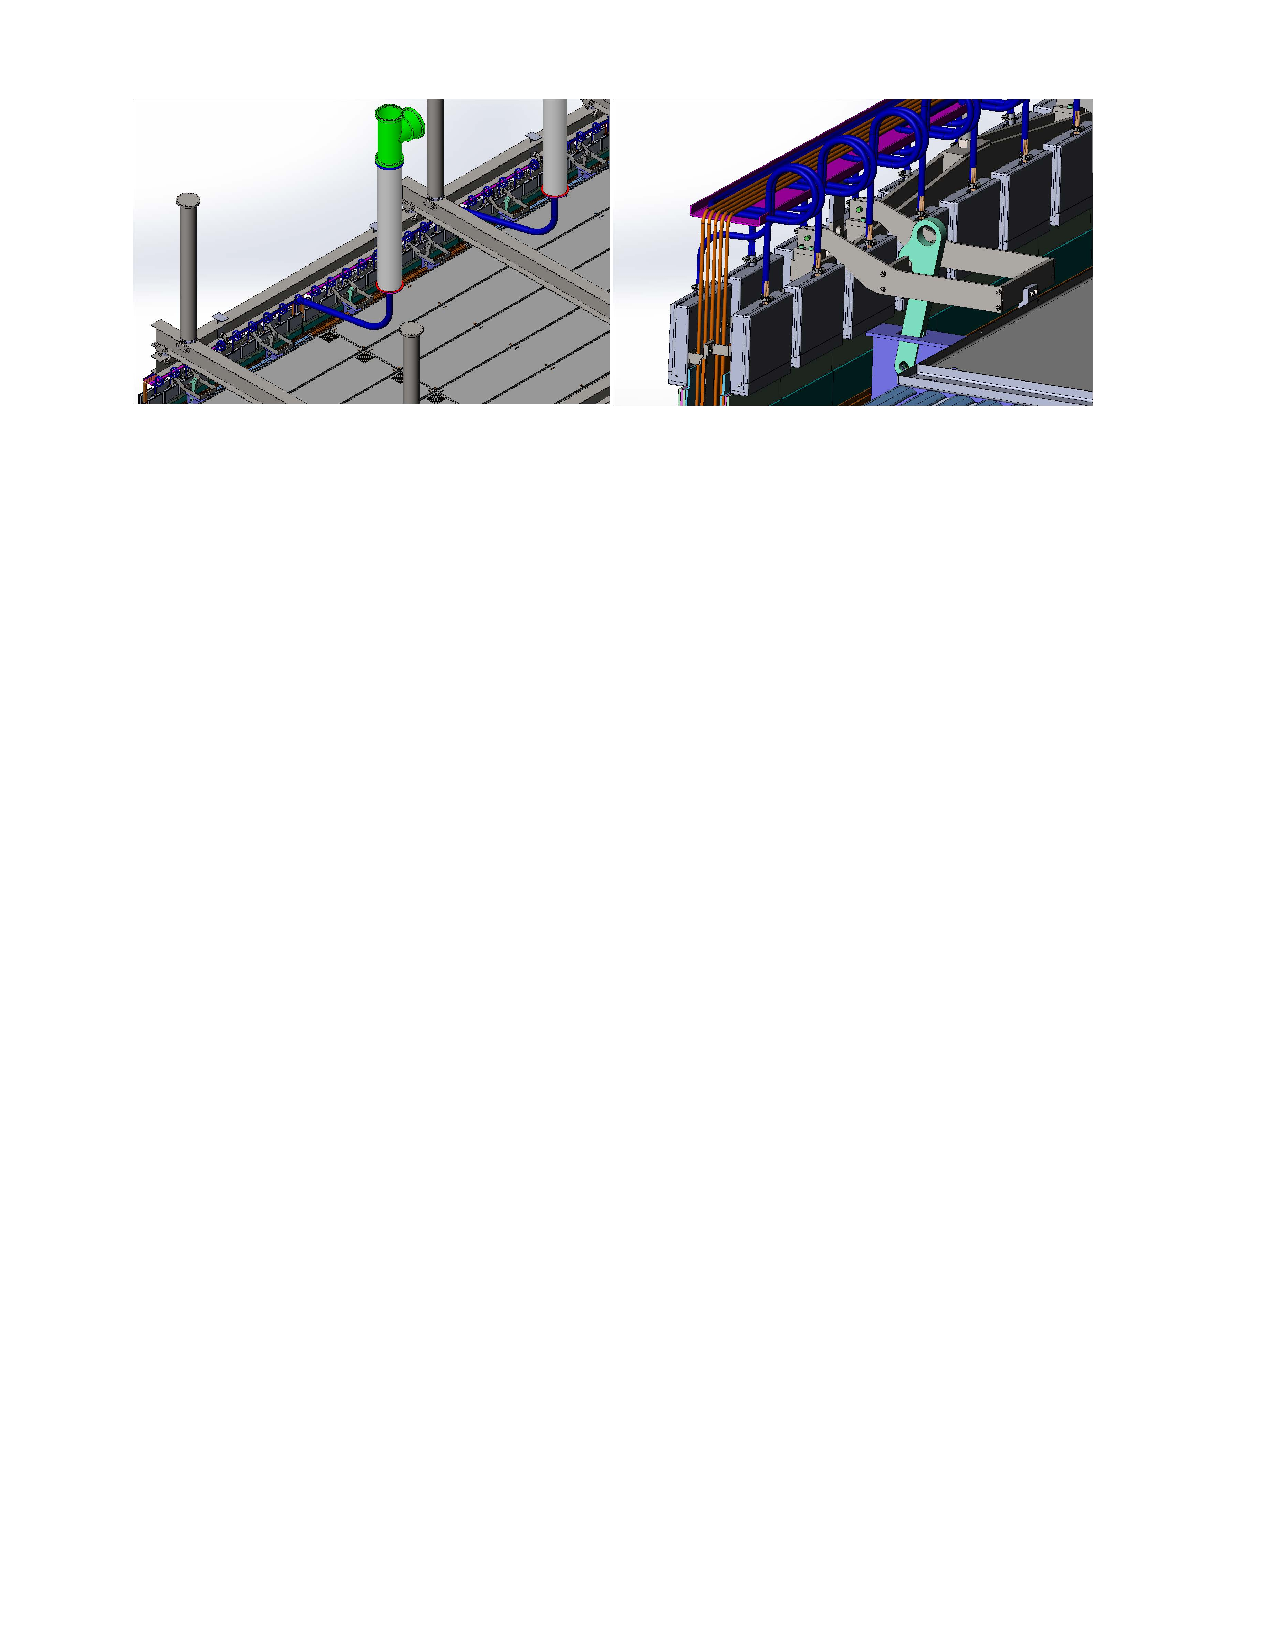
\includegraphics[width=7in]{tpcce_FT_InternalCableRoute.pdf}
\end{cdrfigure}


\begin{cdrfigure}[Conceptual design of signal/power feedthrough]{tpcce_signal_FT}{
TPC signal/power feedthrough. The WIBs are seen edge-on in the left panel,
and in an oblique side-view in the right panel, which also shows the warm crate for a DUNE module in a cutaway view (for 
ProtoDUNE-SP, there is a crate only on one side).}
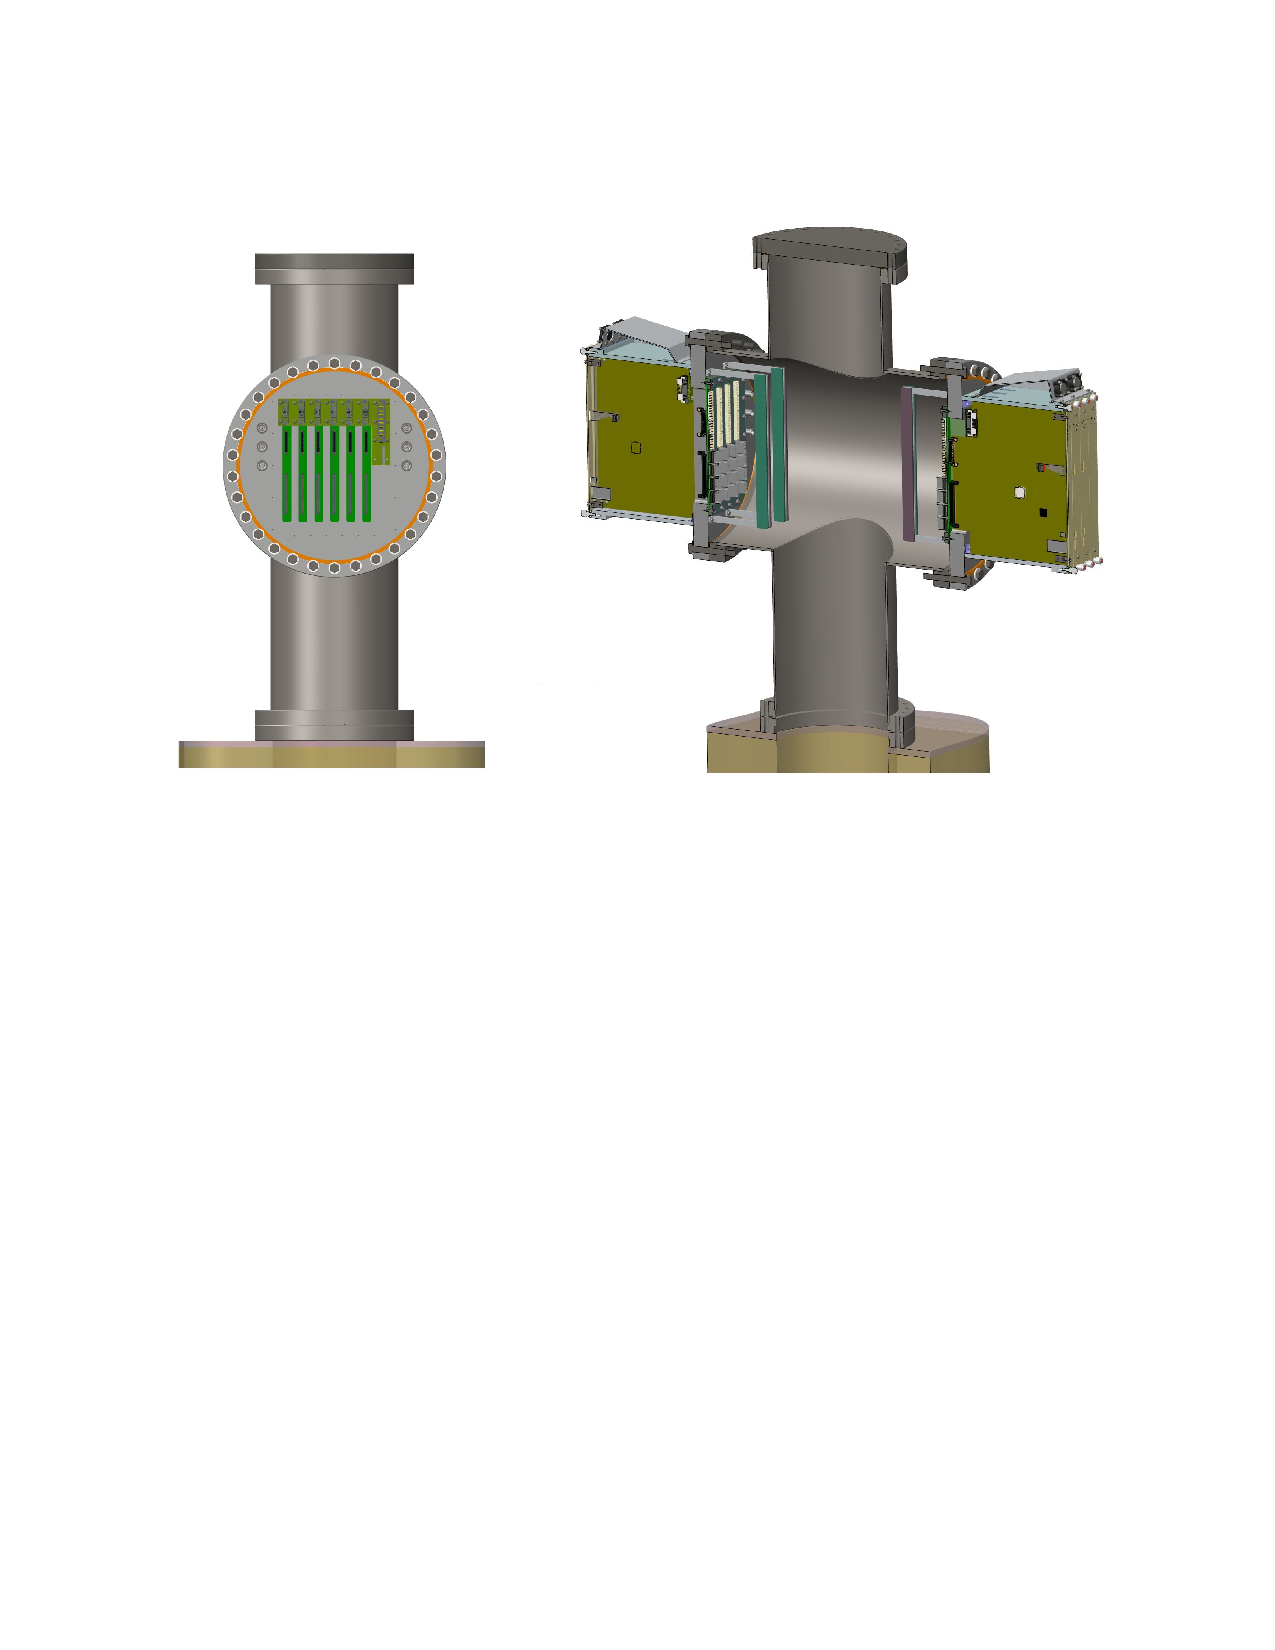
\includegraphics[width=0.6\linewidth]{tpcce_signal_FT.pdf}
\end{cdrfigure}

The current design of the CE flange includes a T-shaped pipe, separate PCB feedthroughs for the CE and PDS cables, and
an attached crate for the TPC warm electronics, as shown in Figure~\ref{fig:tpcce_signal_FT}.
The wire-bias voltage cables connect to standard SHV connectors machined directly into the CE feedthrough,
ensuring no electrical connection between the wire-bias voltages and other signals passing through the CE flange.
Each CE feedthrough serves the bias/power/digital IO needs of one APA, as shown 
in Figure~\ref{fig:tpcce_cable_routing}.  

\begin{cdrfigure}[TPC cable routing scheme]{tpcce_cable_routing}{TPC cable routing scheme for three APA section.}
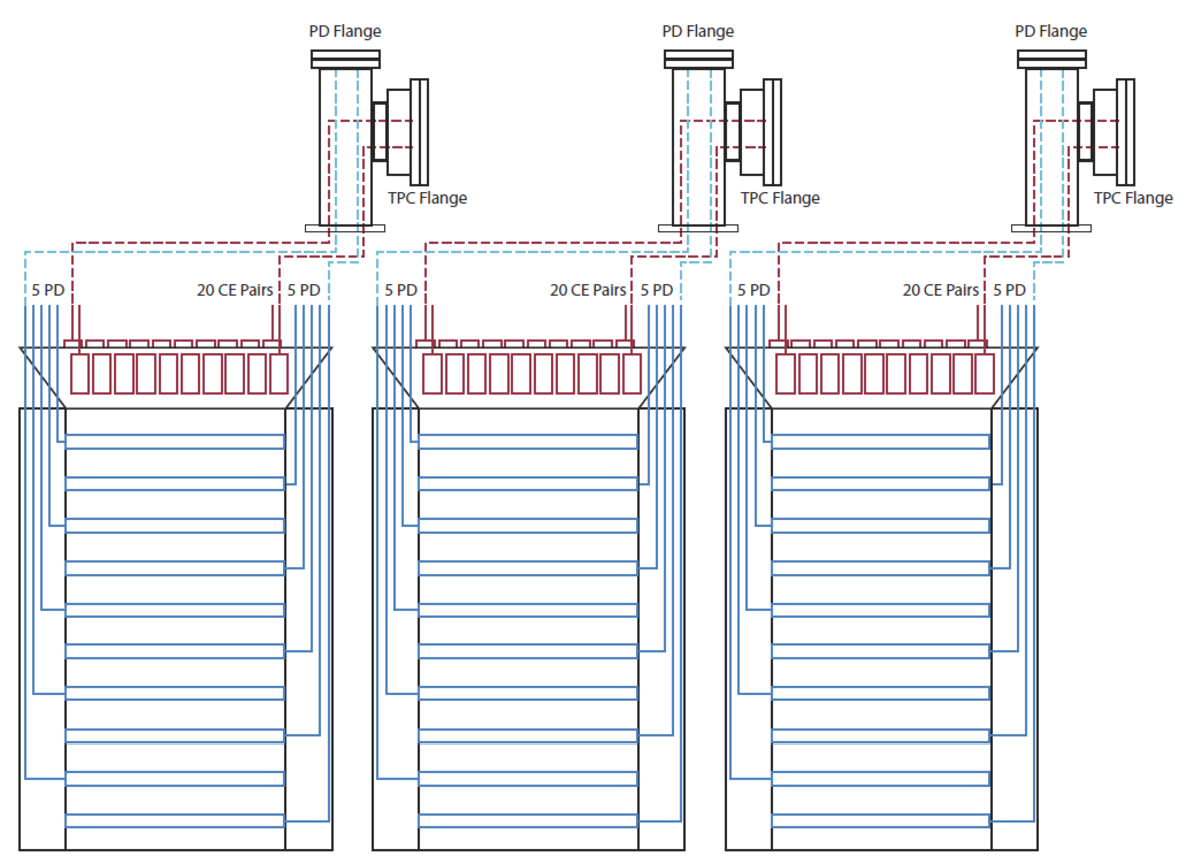
\includegraphics[width=0.9\linewidth]{tpcce_cable_routing.pdf}
\end{cdrfigure}

A program for minimizing potential contamination of the LAr from the cable plant contained within the ullage
(the warmer gas phase at the top of the cryostat) 
is being carefully followed.


Data/control cable bundles are used to send system clock and control signals from the 
CE flange to the FEMB, stream the $\sim$1~Gbps high-speed data from the FEMB to the CE flange, and 
provide backup JTAG programming to the cold FPGA, in case the power-up programming from the onboard 
EEPROM fails. As described in Section~\ref{subsec:ce_intro}, each FEMB 
connects to a CE flange via one data cable bundle, leading to 20 bundles between one APA and one flange.
Each data bundle contains 12 low-skew copper twin-axial cables with a drain wire, 
to transmit the following differential signals:

\begin{itemize}
    \item 4$\times$1.2~Gbps high-speed data
    \item One 50~MHz system clock
    \item One 2~MHz CONVERT clock
    \item 2 I2C control and configure
    \item 4 single-ended JTAG programming for the FPGA
\end{itemize}


\fixme{Figure~\ref{fig:tpcce_samtec_cable} is too detailed to be helpful. Can we crop a part or parts of it?} 

The selected cables are Samtec 26~AWG twin-axial bundles with Samtec HSEC08 connectors to both
the FEMB mezzanine board and the CE flange. 
The HSEC08
connectors lock into place with tabs on each side of the connector. A sample of the Samtec cable with
THV outer jacket has passed outgassing tests in the LAr Materials Test Stand at Fermilab.

The Samtec 26~AWG cable has been
tested and demonstrated to have low enough dispersion such that both the LVDS 50~MHz system clock and
$\sim$1~Gbps high-speed data can be recovered over 25~meters of RT cable, 
significantly longer than the required seven meters needed to run cables between the FEMBs and CE flanges.

\begin{cdrfigure}[Results from cable validation testing]{tpcce_samtec_results}{Eye diagrams 
from cable validation testing. {\bf Top Left:} 50~MHz system clock over 25~m RT  
(RT) Samtec 26AWG cable. For comparison, {\bf Bottom Left} shows the same clock over 
the heavier, prohibitively expensive Gore 24AWG cable. {\bf Top Right:} 1~Gbps data over 
7~m (ProtoDUNE length) RT Samtec 26AWG cable without active recovery by equalizers. {\bf Bottom Right} 1~Gbps
data over 25~m (DUNE length) RT Samtec 26AWG cable with active recovery.}
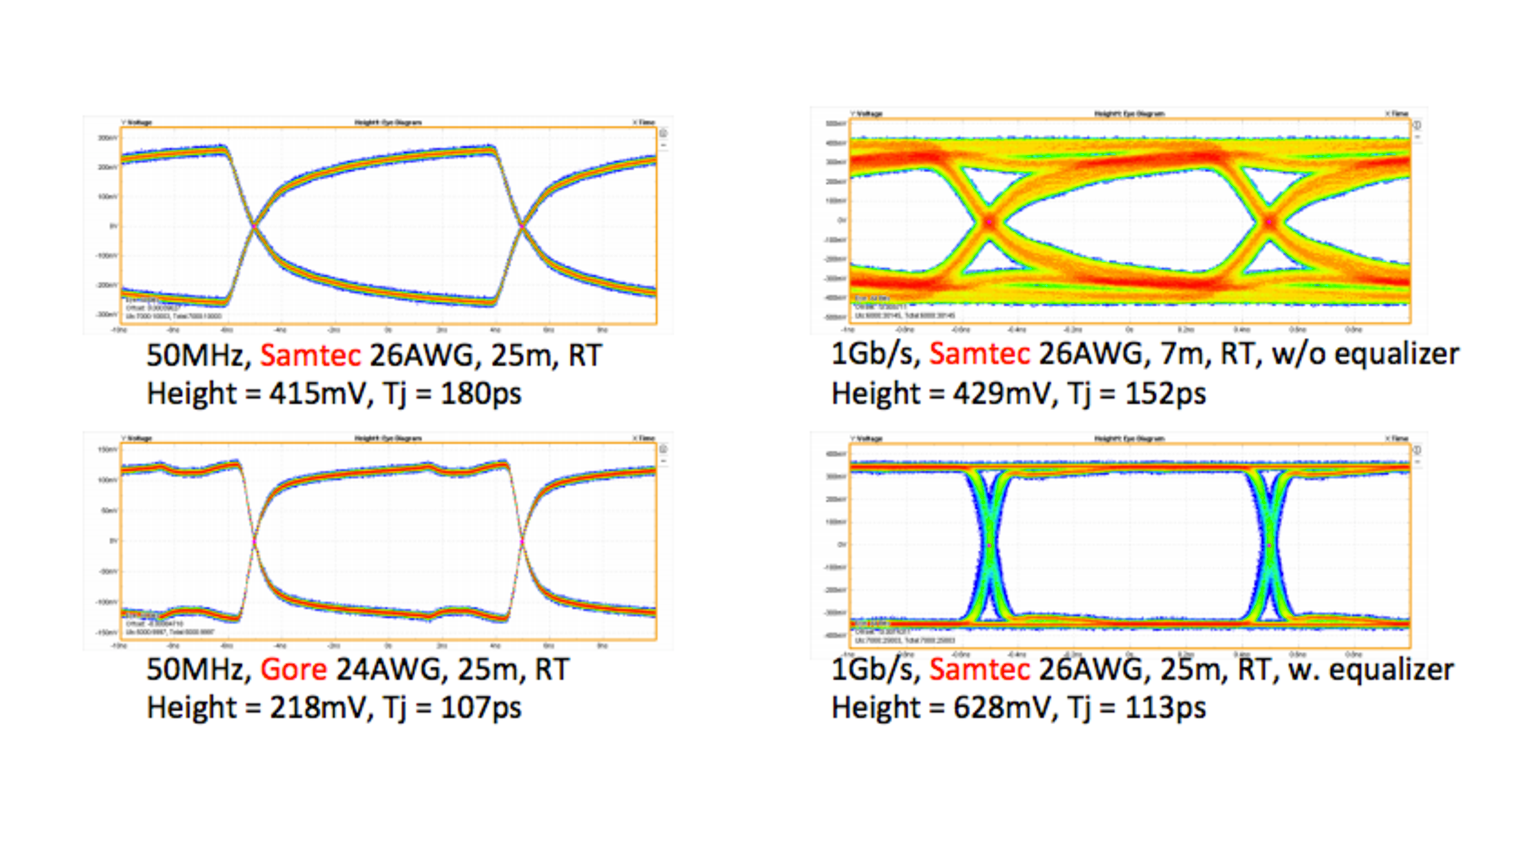
\includegraphics[width=0.9\linewidth]{tpcce_samtec_results.pdf}
\end{cdrfigure}

Figure~\ref{fig:tpcce_samtec_results} shows results from the cable 
validation testing. The eye diagrams show the edges of the differential signals after 
LVDS transmission over the specified cable types and lengths. The height of eye diagram shows the size 
of the recovered signal in mV and the slope of the rising and falling edges are jitter in picoseconds (ps). 
An eye diagram is sufficient to show that the edges of the differential signals can
be recovered, but not enough to demonstrate the bit error rate (BER). However, the Samtec 26~AWG cable has 
also passed a BER test, transmitting $10^{13}$ bits without error.



LV power is passed from the CE flange to the FEMB by bundles of 16 Samtec 
20~AWG twisted-pair wires, as shown in Figure~\ref{fig:tpcce_samtec_cable}. One IPD1 connector
attaches all 16 wires at the CE flange, and two IPD1 connectors are attached to the FEMB (one to the
analog motherboard and one to the FPGA mezzanine). In total, 20 wire bundles 
 bring LV power to the FEMBs associated with one APA.

Eight of the 16 wires are power feeds, as described in Figure~\ref{fig:tpcce_lv_req}. The other eight wires
are attached to the common of the input amplifier circuits, as described in Section~\ref{subsec:ele_design}. For
a single FEMB, the resistance is $<30$~m$\Omega$ at RT or $<10$~m$\Omega$ at LAr temperature. Each APA has a copper cross-section of approximately $80~\mathrm{mm}^2$, with
a resistance $<1.5$~m$\Omega$ at RT or $<0.5$~m$\Omega$ at LAr temperature.

\begin{cdrfigure}[LV power feed wire specifications]{tpcce_lv_req}{Samtec LV power feed wire 
specifications.}
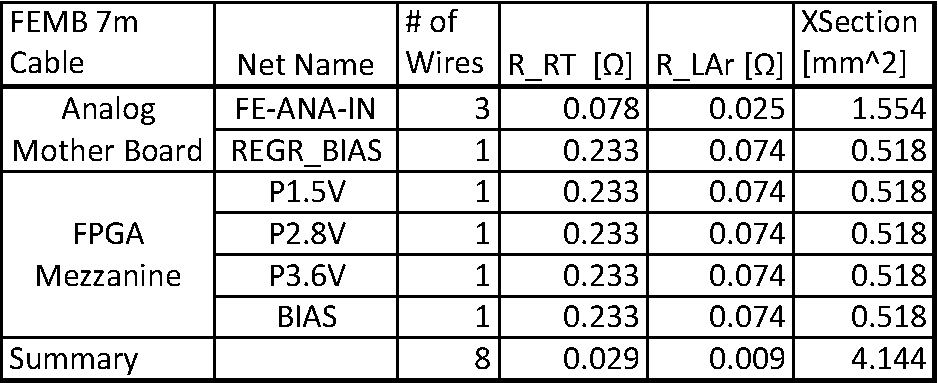
\includegraphics[width=4in]{tpcce_lv_req.pdf}
\end{cdrfigure}

\fixme{Eric questions whether figure~\ref{fig:tpcce_lv_req} is needed}

The wire-bias cable voltages are required to deliver voltages up to a few thousand Volts and currents up to a few
milliAmps.

The bias voltages are applied to the X-, V-, and G-plane wire layers, three field cage terminations, 
and an electron diverter, as shown in Figure~\ref{fig:tpcce_cr_board}. The voltages are supplied 
through eight SHV connectors mounted on the CE flange. RG-316 coaxial cables carry the voltages 
from the CE flange to a patch panel PCB which includes noise filtering mounted on the top 
end of the APA. 

From there, wire-bias voltages are carried by single wires to 
various points on the APA frame, including the CR boards, a small PCB mounted on or near 
the patch panel that houses a noise filter and termination circuits for the field cage voltages, and 
a small mounted board near the electron diverter that also houses wire-bias voltage filters.


%%%%%%%%%%%%%%%%%%%%%%%%%%%%%%%%    
\subsection{Warm interface electronics}
\label{subsec:warm_interface_elec}

The warm interface electronics are housed in a small crate
attached directly to the cryostat flange.  The crate contains one
Power and Timing Card (PTC), up to five Warm Interface Boards (WIBs) and a passive
backplane (PTB), which fans out signals and LV power from the PTC to the WIBs.

\begin{cdrfigure}[Conceptual design of CE flange]{tpcce_ceflange_sbnd}{Exploded view of 
the CE flange for SBND (ProtoDUNE has 5 WIBs).}
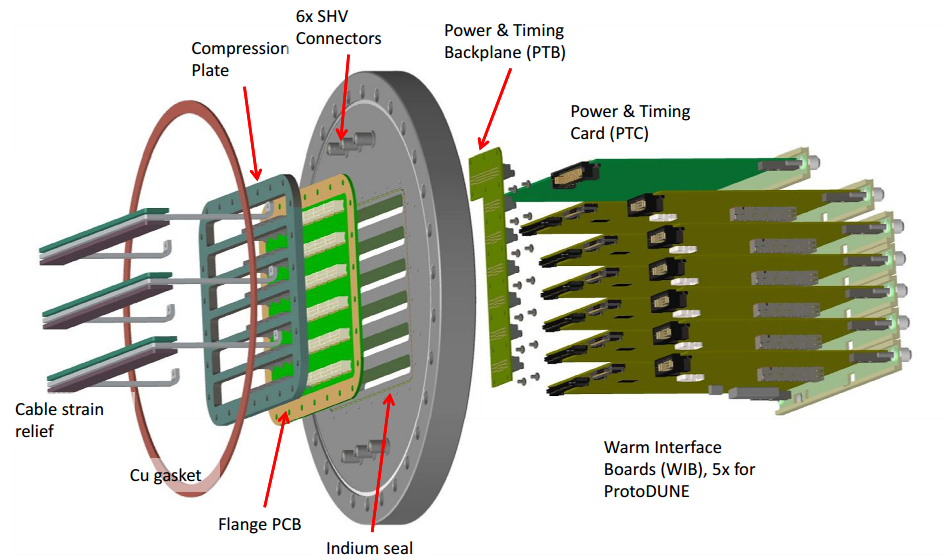
\includegraphics[width=0.9\linewidth]{tpcce_ceflange_sbnd.png}
\end{cdrfigure}

The WIB is the interface between the
DAQ system and up to four
FEMBs. It receives the system clock and control signals from the
timing system and provides for processing and fan-out of those signals to the four
FEMBs. The WIB also receives the high-speed data signals from the four 
FEMBs and transmits them to the DAQ system over optical
fiber.  Figure~\ref{fig:tpcce_ceflange_sbnd} shows the TPC warm electronics
flange. The WIBs are attached directly to the TPC
readout electronics feedthrough on the CE flange. The feedthrough
board is a PCB with connectors to the cold signal and LV cables fitted
between the compression plate on the cold side, and sockets for
the WIB on the warm side. Cable strain relief is also provided
directly on the CE flange.

%%%%%%%%%%%%%%%%  
%\subsubsection{Power and Timing Card}
%\label{subsubsec:power_timing_card}

\begin{cdrfigure}[PTC and timing]{tpcce_wib_timing}{Power and Timing Card (PTC) 
and timing distribution to the WIB and FEMBs.}
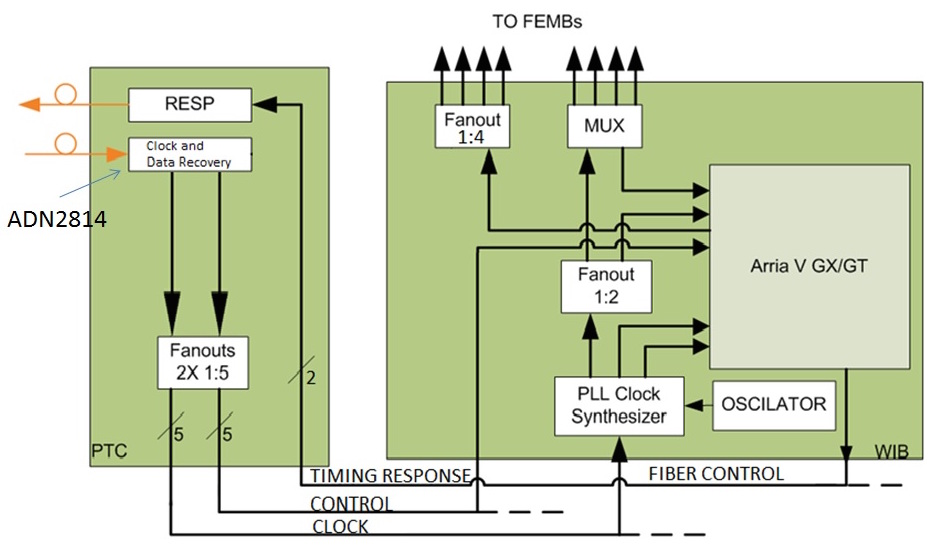
\includegraphics[width=0.5\linewidth]{tpcce_wib_timing.jpg}
\end{cdrfigure}

The PTC provides a bidirectional fiber interface to the
timing system.  The received data is separated into clock and
data using a clock/data separator.  The clock and data
streams are separately fanned-out to the five WIBs as shown in
Figure~\ref{fig:tpcce_wib_timing}. The PTC fans the clocks out to the WIB over the
PTB, which is a passive backplane attached directly to the PTC and
WIBs. See Figures~\ref{fig:tpcce_ceflange_sbnd} and~\ref{fig:tpcce_dune_ptb}.

\begin{cdrfigure}[WIB and LV power]{tpcce_wib_power}{LV power distribution 
to the WIB and FEMBs. 200W is for a fully-loaded crate 
with the majority of the power dissipated by the 20 cold FEMBs in the LAr.}
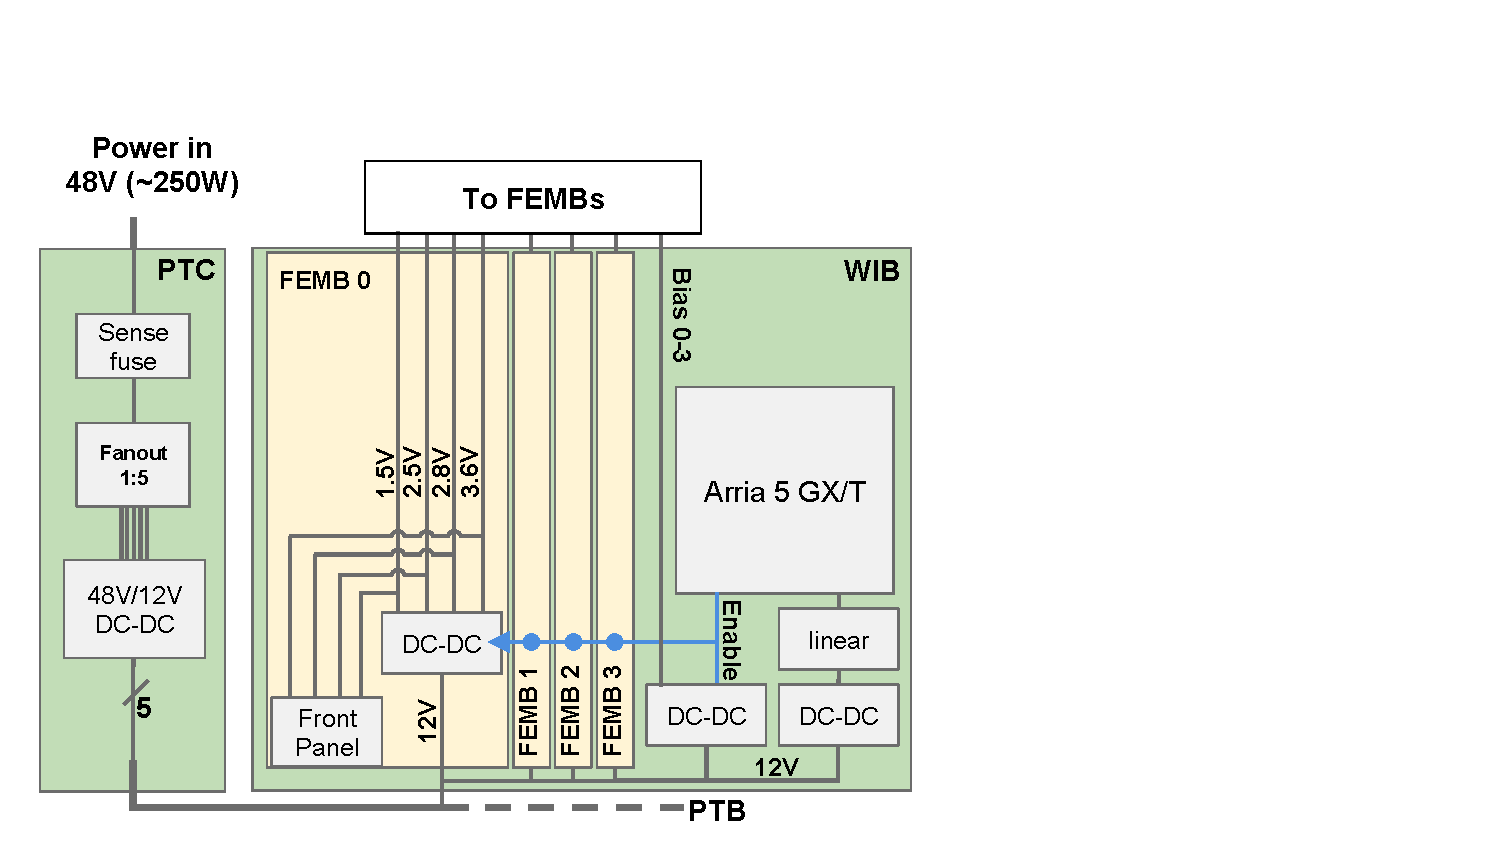
\includegraphics[width=0.6\linewidth]{tpcce_wib_power.pdf}
\end{cdrfigure}

The PTC also receives LV power for all cold
electronics connected to that flange, approximately 200W at 12V for a
fully-loaded flange (5~WIB + 20~FEMB). The LV power is then fanned out
on the PTB to each WIB, which provides the necessary DC/DC conversions and fans
the LV power out to each of the cold FEMBs supplied by that WIB, 
as shown in Figure~\ref{fig:tpcce_wib_power}. The 
majority of the 200W drawn by a full flange is dissipated in the LAr
by the cold FEMB.


%%%%%%%%%%%%%%%%  
%\subsubsection{Warm Interface Board}
%\label{subsubsec:warm_interface_board}

Each WIB contains a 
unique IP address for its UDP slow control interface. The IP address for the WIB is 
derived from a crate and slot address: the crate address is generated on the PTC 
board via dipswitches and the slot address is generated by the PTB slot, numbered 
from one to five. Note that the WIB also has front-panel
connectors for receiving LV power, which can be used in place of the LV power inputs on the PTB generated by the PTC.

The WIB is also capable of
receiving the encoded system timing signals over bi-directional optical
fibers on the front panel, and processing these using either
the on-board FPGA or clock synthesizer chip to provide the 50~MHz
clock required by the cold electronics.  

\begin{cdrfigure}[Warm Interface Board]{tpcce_dune_wib}{Warm interface board (WIB). Note 
that front panel inputs include a LEMO connector and alternate inputs for LV power.}
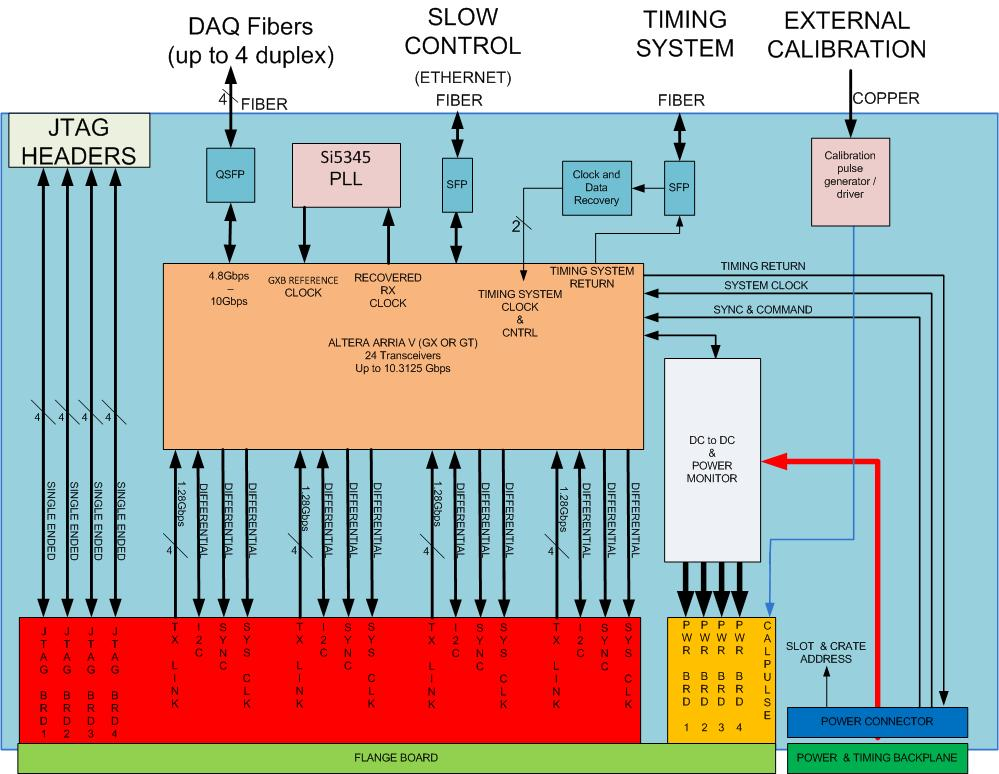
\includegraphics[width=0.9\linewidth]{tpcce_dune_wib.jpg}
\end{cdrfigure}

The FPGA on the WIB is an Altera Arria V GT variant, which requires a
125~MHz clock for its state machine that is provided by an on-board crystal
oscillator. The GT variant of the Arria V
transceivers can drive the high-speed data to the DAQ system up to
10.3125~Gbps per link,  implying that all data from
two FEMB (2$\times$5~Gbps) could be transmitted on a single link. However, it is planned to
use a QSPF socket on the WIB to deliver $\sim$5~Gbps on four optical fibers 
(one fiber per FEMB) to two RCEs. \fixme{write out} The FPGA has an additional Gbps Ethernet
transceiver I/O based on the 125~MHz clock, which provides real-time digital data readout to slow control.



%
%%%%%%%%%%%%%%%%%%%%%%%%%%%%%%%%  
\subsection{External Power and Cables}
\label{subsec:ce_feedthrough_power}

The LV power to the FEMB and WIB is supplied by Weiner MPOD power supplies. 
The CE power-per-channel is about 25~mW in the LAr.
Including power for the WIB, a fully loaded WIB (one WIB plus four FEMBs) requires
12V and draws approximately 3.3~Amps. Therefore, the full electronics for one APA (five WIBs + 20 FEMBs) 
requires 12~V and draws approximately 16~Amps, for a total power of almost 200~W, as 
described in Section~\ref{subsubsec:power_timing_card}.

Each MPOD LV unit has two DSUB37 connectors, each with 4 channels of LV output, including negative
and positive sense wires. %as shown in Figure~\ref{fig:tpcce_mpod_top}. 
Each channel has three pins
of negative output and three pins of positive output. Five of the eight channels
provide the 12~V/3.3~A to each WIB via the PTC, and one channel provides LV power 
to the PTC itself, with two of the eight channels unused.

%\begin{cdrfigure}[MPOD DSUB37 top connector]{tpcce_mpod_top}{MPOD DSUB37 top connector.}
%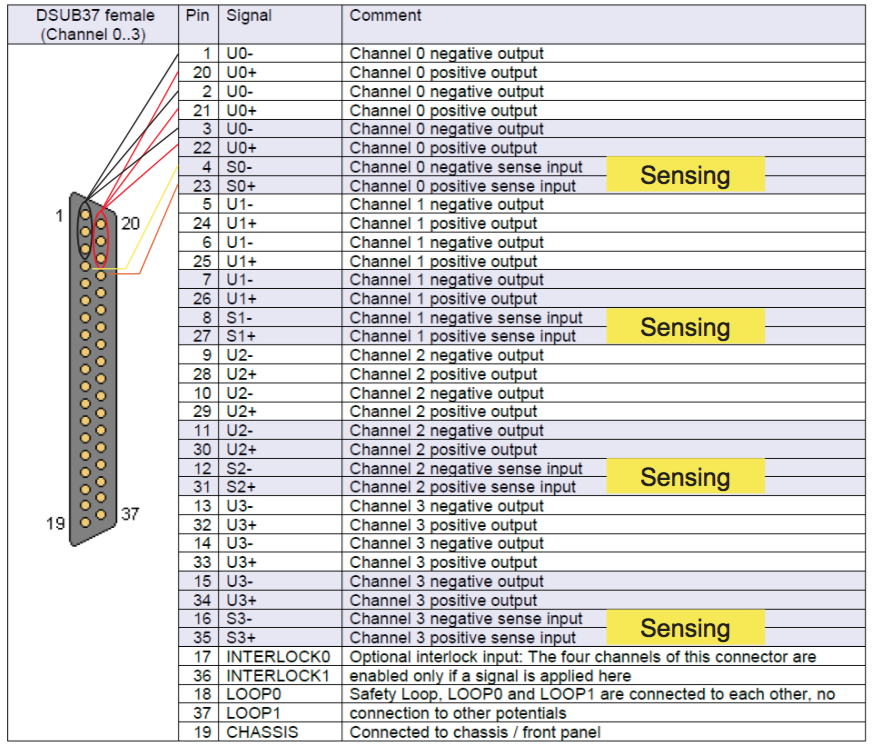
\includegraphics[width=1.0\linewidth]{tpcce_mpod_top.png}
%\end{cdrfigure}

Each MPOD wire-bias voltage unit supplies the wire-bias voltage to eight SHV connectors 
at the CE flange. One MPOD chassis contains three LV and three wire-bias units, and can
supply all the LV and wire-bias power to three APAs worth of cold electronics. Therefore,
a total of two MPOD chassis are required for the ProtoDUNE-SP detector.

%
%%%%%%%%%%%%%%%%
%\subsubsection{Low-voltage cable}
%\label{subsubsec:ce_feedthrough_lv}

The LV cable uses DSUB37 connectors. The bottom of the fuse PCB at the MPOD 
end of the cable is shown in Figure~\ref{fig:tpcce_fused_cable}. Each of the three output pins on
each channel are tied together in parallel 
going to one wire large enough to carry the full supply voltage. Fuses can optionally be 
populated on each output pin as shown in Figure~\ref{fig:tpcce_fused_cable}; however, if
fusing is not selected, the pins will be connected with 0~$\Omega$ resistors. This fusing would serve as
a final protection. The primary protection would come from the Over Current protection
on the MPOD, which is set above the 3.3~A required by each WIB, but below the
combined fuse value.

\begin{cdrfigure}[Bottom of the fuse PCB]{tpcce_fused_cable}{Bottom of the fuse PCB at the MPOD end of the cable.}
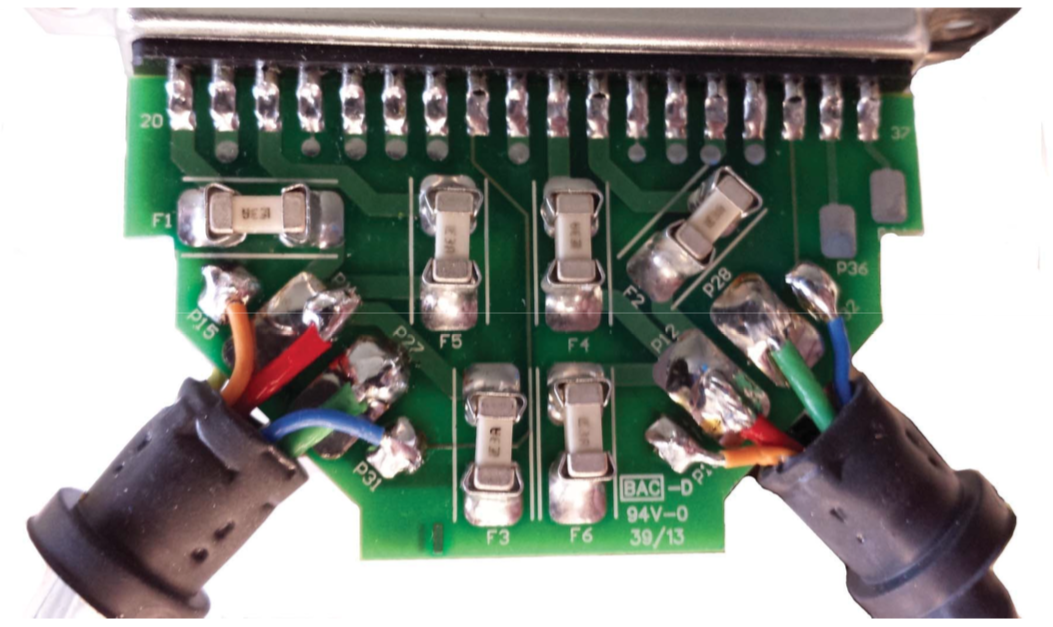
\includegraphics[width=0.7\linewidth]{tpcce_fused_cable.png}
\end{cdrfigure}

The five separate 12~V/3.3~A channels to the WIBs are delivered to the PTC using two normal DSUB37 connectors to
attach the LV power cable. The fusing for the sense wires is implemented on the PTC.

%
%%%%%%%%%%%%%%%%
\subsubsection{Wire Bias Voltage Cable}
\label{subsubsec:ce_feedthrough_wirebias}

Each anode plane assembly requires three bias voltage connections 
at $+$820V, $-$370V, and $-$665V, as described in Section~\ref{subsec:ce_wire_bias}.
The current on each of these supplies is expected to be zero at normal operation.
However the ripple voltage on the supply must be carefully controlled 
to avoid noise injection into the front-end electronics.

RG-58 coaxial cables connect the wire bias voltages from the MPOD to the standard SHV
connectors machined directly into the flange, so there is no electrical connection between 
the LV and data connectors and bias voltage. The length of the cables from the Weiner MPODs
to the CE flanges is estimated to be 18~meters.

%
%%%%%%%%%%%%%%%%
\subsubsection{Optical Fiber}
\label{subsubsec:ce_optical_fiber}

Optical fiber provides the connections between the warm electronics crate, which acts as
a Faraday-shielded box, to the DAQ and slow control systems.
Each WIB uses QSFP sockets for 
four pairs of fiber, as described in Section~\ref{subsubsec:warm_interface_board}, 
implying a total of 120 optical data fibers for the 30 WIB boards in the system. The optical fibers from
the CE flanges to the DAQ room are an estimated 30$-$40~m in length.

Duplex LC optical fiber is under consideration for transmitting the one GIG-E connection from each
WIB to slow control. The WIB reports the current draw from each FEMB to the slow control system, while the 
current draw for each WIB is monitored at the MPOD itself.

